\section{DPS u krbů}
\label{sec:dps-u-krbu}
Navržená DPS se skládá z části elektronické pojistky TPS2600, zapojení je obdobné jako v \ref{sec:napajeni-1-wire-sbernice} (napájení 1-Wire sběrnice), navíc je na vstupu připojena transilová dioda (ESD9L5.0ST5G). Napěťové meze jsou nastaveny stejně, tedy minimální napětí je 4,75 V, maximální 5,25 V, proud je omezen na maximální hodnotu 100 mA. Dále je zde přivedena 1-Wire sběrnice přes konektor RJ45 s~obdobnými ochranami jako v \ref{sec:datova-cast-1-wire-sbernice} (datová část 1-Wire sběrnice) pro připojení MAX31850K přes svorkovnici. V neposlední řadě jsou zde vstupy pro ovládání třech LED pro signalizaci (obrázek \ref{fig:led-indikace}) naakumulovaného zásobníku otopné vody, modrá led signalizuje stav horní části zásobníku, oranžová LED je pro střední část, červená je pro signalizaci spodní části. Vstupní část je chráněná přes DS9503 a transilovou diodou (ESD9L5.0ST5G). Sepnutí LED je přes tranzistor (BSS138P). Obdobně jsou řešeny oranžová a modrá LED. Celkové schéma zapojení je v~příloze \ref{app:schemata-ostatni}.

\begin{figure}[H]
    \centering
    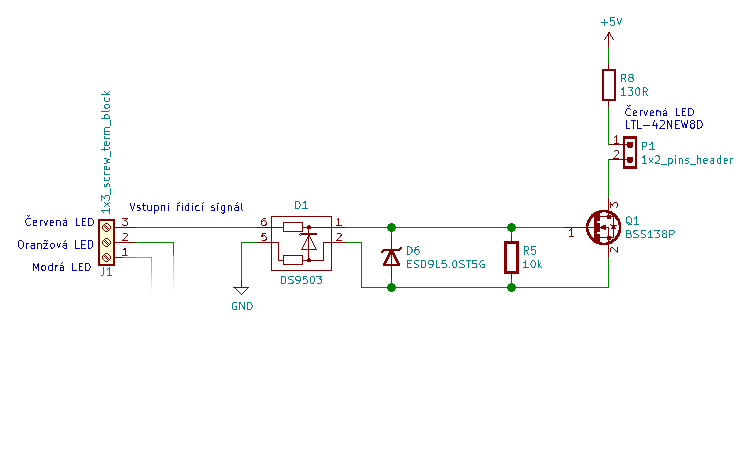
\includegraphics[width=\textwidth]{images/svg/kicad/led-indikace.eps}
    \caption{Zapojení pro ovládání signalizační červené LED.}
    \label{fig:led-indikace}
\end{figure}

\subsubsection{I$^2$C sběrnice}
\label{sec:i2c-sbernice}
Sběrnice I$^2$C je realizovaná pomocí zakoupeného modulu (obrázek \ref{fig:modul-pca9615-i2c-sbernice}) s~obvodem PCA9615 do firmy  NXP Semiconductors. Vstupní signál SCL a~SDA je veden přímo z~centrální jednotky na vstupu obovodu PCA9615, napájení je s 3,3 V logikou. Výstup z PCA9615 je pomocí diferenciální veden. Napájení na této straně je 5 V. Sběrnice je realizovaná pomocí UTP Cat5e, výstup z~modulu je realizován pomocí konektoru RJ45. Vzhledem k použití UTP kabelu a diferenciálnímu přenosu je možné dosáhnout velké vzdálenosti sběrnice. Nejdelší bod dosahuje přibližně 30 m, je tedy možné použít I$^2$C sběrnici na vzdálenost pro kterou není standartě dělána. Použitá frekvence je 100~kHz. Jedná se tedy o plnohodnotnou I$^2$C sběrnici. Důvodem pro zvolení této varianty bylo na základě výběru displeje s I$^2$C sběrnicí (jednoduché a~levné řešení), dále jedná se o klasické zapojení displeje jako by se nalézal v~krátké vzdálenosti od centrální jednotky a není tak nutný převod jako při využít např. RS485 na UART a následně na I$^2$C sběrnici, v neposlední řadě komunikace je definována podle protokolu I$^2$C.  Jeden modul se nalézá na straně centrální jednotky a pak na straně krbů. Napájení 5 V je realizováno pomocí samostatných kabelů, není tedy součástí UTP kabelu. Z důvodu omezení kabeláže je sběrnice realizována v jednom UTP kabelu s 1-Wire sběrnicí, tedy přesněji jsou využity volné vodiče 1,2 pro SCL a~7,~8 pro SDA. Zařízení lze zapojovat jak na straně před PCA9615, tak i~na diferenciální straně, je však výhodné připojené uzly udržet co v nejkratší vzdálenosti kvůli degradování signálu. Blokové schéma je na obrázku \ref{fig:blokove-schema-pca9615-i2c-sbernice} včetně napojení uzlů. Schéma zapojení modulu je na obrázku \ref{fig:zapojeni-pca9615-i2c-sbernice}.

\begin{figure}[H]
    \centering
    \def\svgwidth{\columnwidth}
    \input{images/svg/blokove-schema-pca9615-i2c-sbernice.pdf_tex}
    \caption[Blokové schéma zapojení obvodu PCA9615.]{Blokové schéma zapojení obvodu PCA9615 s impedančním zakončením sběrnice a možnostmi napojení uzlů. Upraveno z \cite{pca9615-schema-zapojeni}.}
    \label{fig:blokove-schema-pca9615-i2c-sbernice}
\end{figure}

\begin{figure}[H]
    \centering
    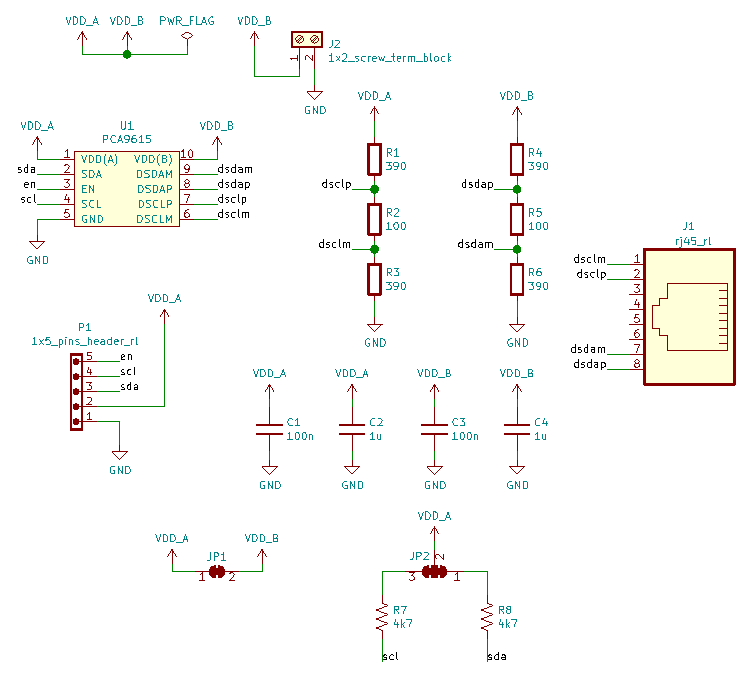
\includegraphics[width=\textwidth]{images/svg/kicad/zapojeni-pca9615-i2c-sbernice.eps}
    \caption[Zapojení PCA9615 v modulu.]{Zapojení PCA9615 v modulu. Upraveno z \cite{pca9615-schema-zapojeni}.}
    \label{fig:zapojeni-pca9615-i2c-sbernice}
\end{figure}

Výhodou PCA9615 je automatický výběr směru komunikace, není potřeba externího ovládání. Komunikace je možná až do rychlosti 1 MHz (přibližně pro 3 m), se zvýšenou délkou je však nutné rychlost snížit. Komunikace využívá standardního protokolu I$^2$C. Nezávislost napájení, je možné napájet koncová zařízení z jiného zdroje než Master. V neposlední řadě se jedná o jednoduché řešení bez nutných další zařízení na straně Slave, stačí pouze zapojit koncové zařízení s~podporou I$^2$C. Na obrázku \ref{fig:modul-pca9615-transily} jsou pro větší ochranu modulu přidány obousměrné transil diody (SM6T6V8CAY) připájené na vstupní piny konektoru RJ45 (obvod sám o sobě poskytuje vstupní ochranu pro ESD). Pro rozbočení I$^2$C sběrnice do jednotlivých pater slouží DPS s konektory RJ45 (schéma viz příloha \ref{app:schemata-ostatni}, obrázky viz příloha \ref{app:rozbocovac-i2c}).

\begin{figure}[H]
    \centering
    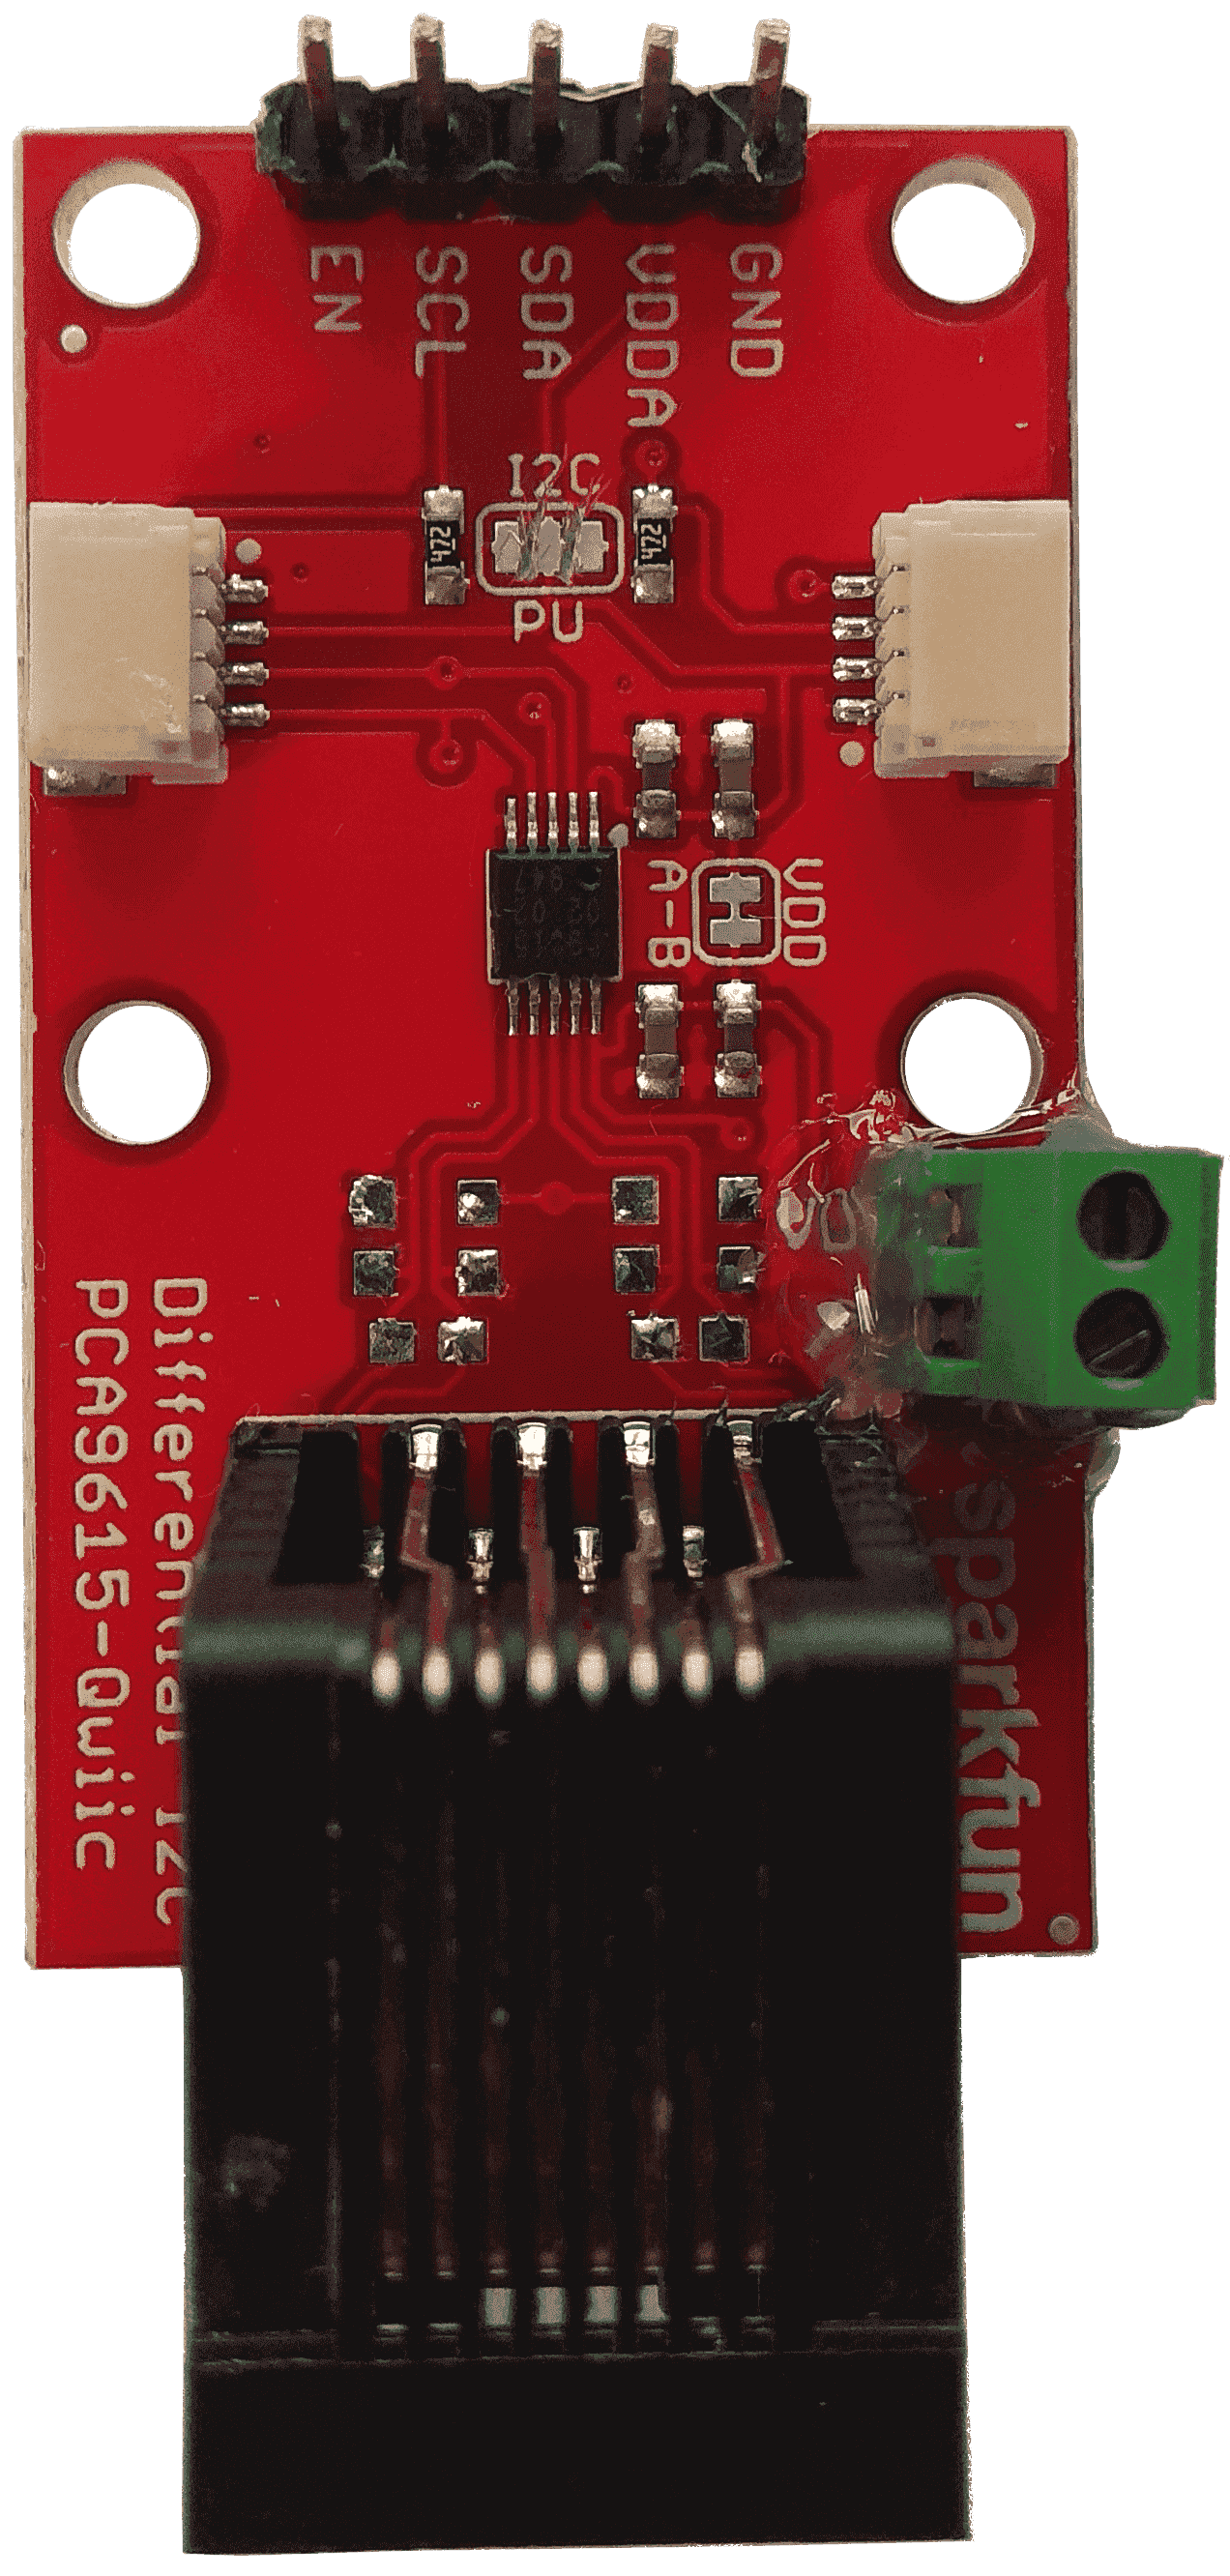
\includegraphics[width=0.7\textwidth]{images/krb/modul-pca9615-i2c-sbernice.png}
    \caption[Modul s obvodem PCA9615.]{Modul s obvodem PCA9615.}
    \label{fig:modul-pca9615-i2c-sbernice}
\end{figure}

\begin{figure}[H]
    \centering
    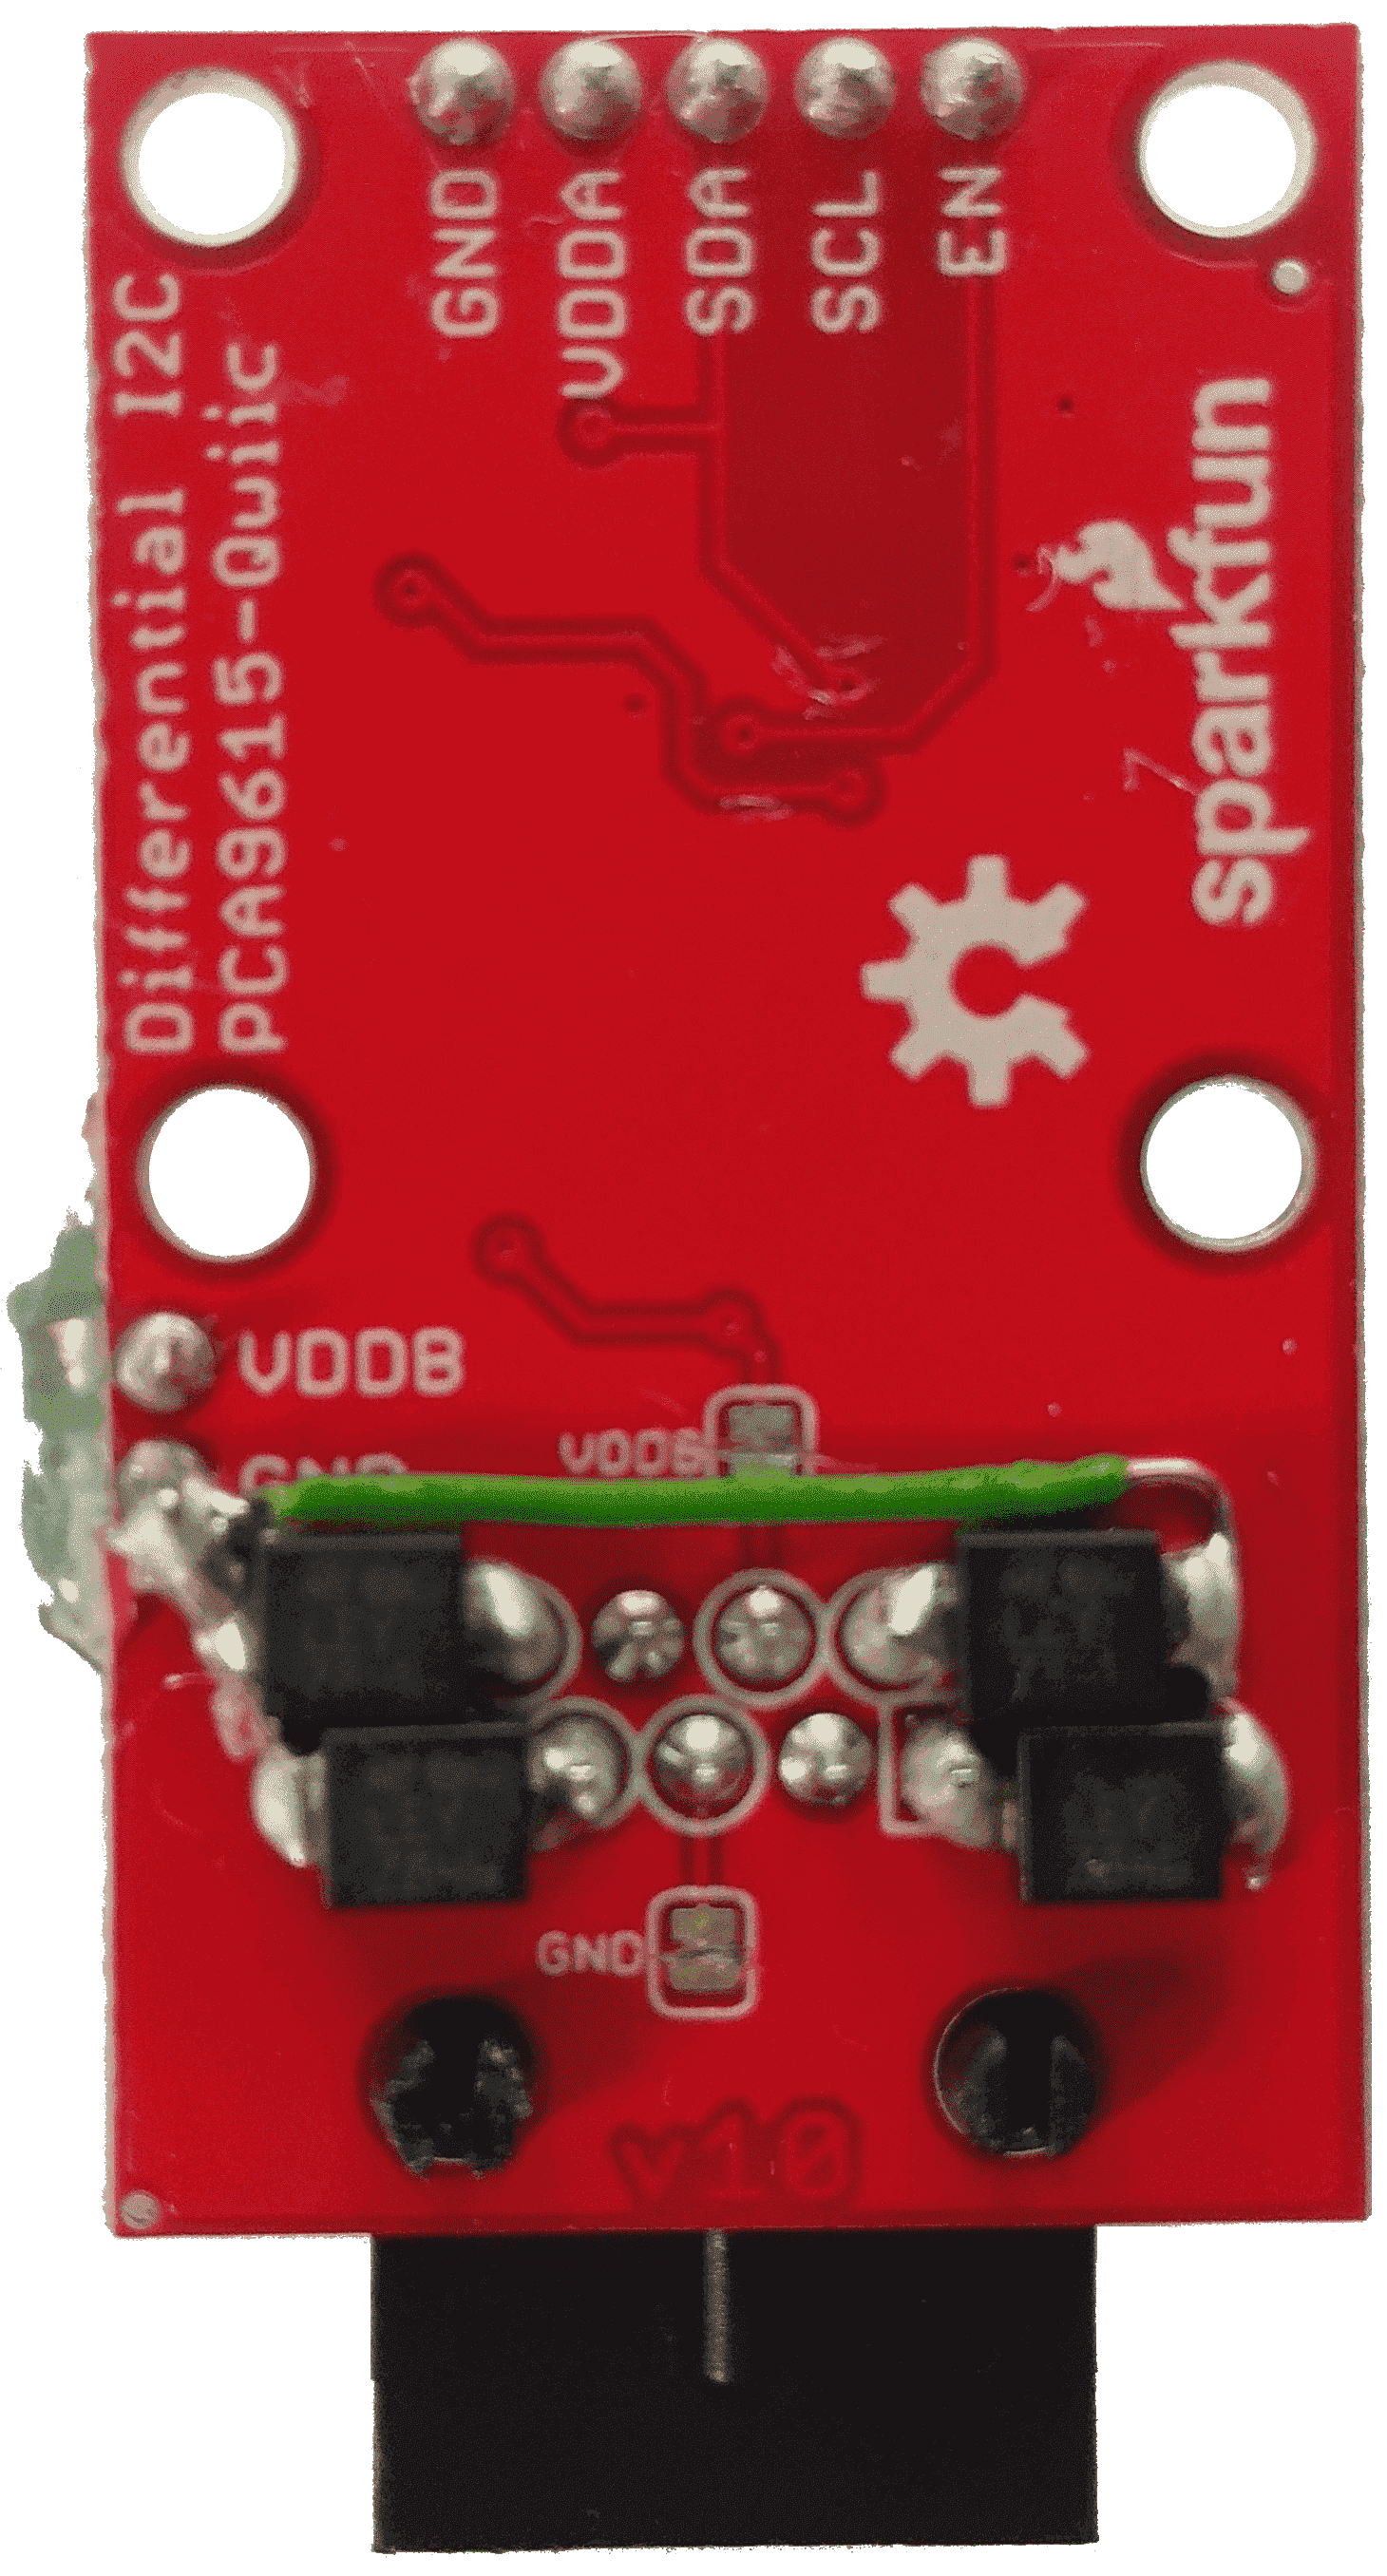
\includegraphics[width=0.6\textwidth]{images/krb/modul-pca9615-transily.png}
    \caption[Modul s obvodem PCA9615 s transily.]{Modul s obvodem PCA9615 s ochrannými transily.}
    \label{fig:modul-pca9615-transily}
\end{figure}


\subsubsection{Měření teploty pomocí termočlánku a převodníku MAX31850K}
Teplotní senzory připojené na kouřovody krbů jsou realizované pomocí termočlánku z \ref{sec:teplotni-senzory-pro-krby}. Termočlánek je připojený k zakoupenému modulu (obrázek~\ref{fig:modul-max31850k-1-wire-prevodnik-termoclanku}), hodnota napětí z termočlánku je převedena do digitální podoby včetně teplotní kompenzace studeného konce a~tato hodnota je poslána po 1-Wire sběrnici. Je možné připojit termočlánek typu K. Převodník umožňuje měřit teplotu s~převodem pomocí AD převodníku až na 14 bitů. Rozlišení teploty činí 0,25~°C. Při teplotách -200 °C až 700 °C činí přesnost měřené teploty ±2~°C. Obvod disponuje detekcí zkratu (na GND nebo napájení) na vstupu pro termočlánek. Dále je zde detekci odpojeného termočlánku. Schéma zapojení modulu je na obrázku \ref{fig:zapojeni-max31850k-1-wire-prevodnik-termoclanku}.

\begin{figure}[H]
    \centering
    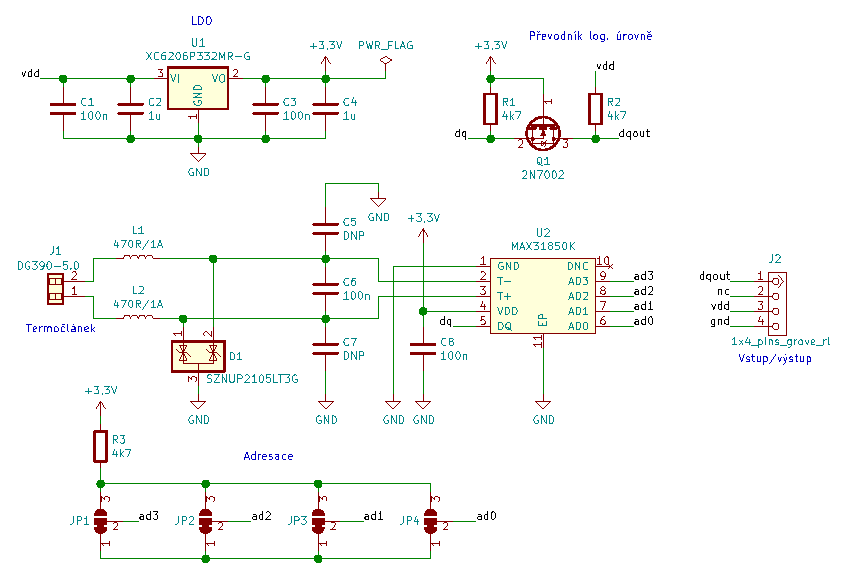
\includegraphics[width=\textwidth]{images/svg/kicad/zapojeni-max31850k-1-wire-prevodnik-termoclanku.eps}
    \caption[Zapojení MAX31850K v modulu.]{Zapojení MAX31850K v modulu. Upraveno z \cite{prevodnik-max31850k}.}
    \label{fig:zapojeni-max31850k-1-wire-prevodnik-termoclanku}
\end{figure}

\begin{figure}[H]
    \centering
    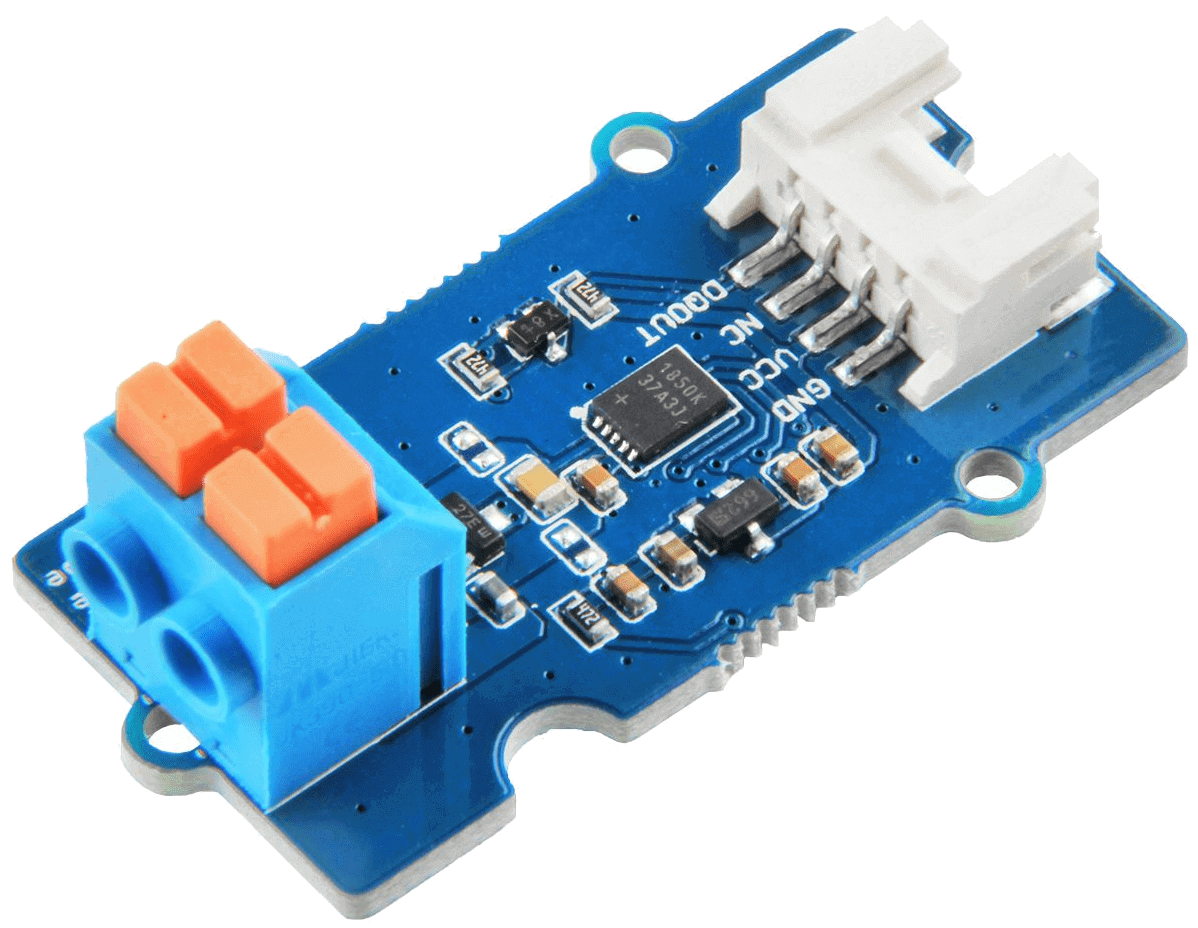
\includegraphics[width=0.6\textwidth]{images/krb/modul-max31850k-1-wire-prevodnik-termoclanku.png}
    \caption[Modul s obvodem MAX31850K.]{Modul s obvodem MAX31850K \cite{prevodnik-max31850k}.}
    \label{fig:modul-max31850k-1-wire-prevodnik-termoclanku}
\end{figure}

\subsubsection{LCD displej}
Pro zobrazování teplot ze střední a spodní části zásobníku otopné vody byl zvolen 16 znakový a 2 řádkový LCD displej s modrým podsvícením a~bílými písmeny (obrázek \ref{fig:lcd-displej}). Po obsluhu displeje slouží řadič HD44780. K~řadiči je připojen I$^2$C expandér PCF8574 s osmi výstupy, které jsou připojená na datovou sběrnici pro ovládání respektive zobrazování znaků na displeji. Displej je zapojen za modulem popsaným v části \ref{sec:i2c-sbernice} (I$^2$C sběrnice). Každý displej, respektive expandér PCF8574 umožňuje nastavit pomocí propojek A0, A1, A2 unikátní adresu zařízení na sběrnici.

\begin{figure}[H]
\centering
\begin{subfigure}{.5\textwidth}
  \centering
  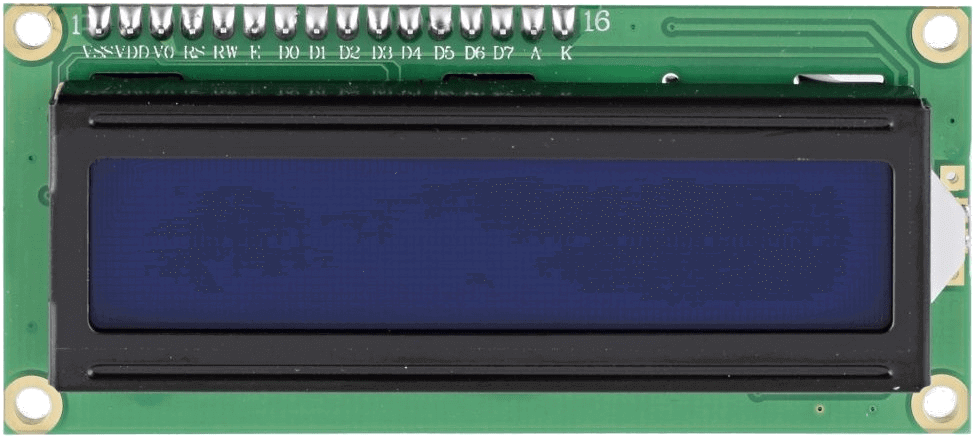
\includegraphics[width=0.91\linewidth]{images/krb/predni-cast-lcd-displeje.png}
  \caption{Přední část displeje.}
  \label{fig:predni-cast-lcd-displeje}
\end{subfigure}%
\begin{subfigure}{.5\textwidth}
  \centering
  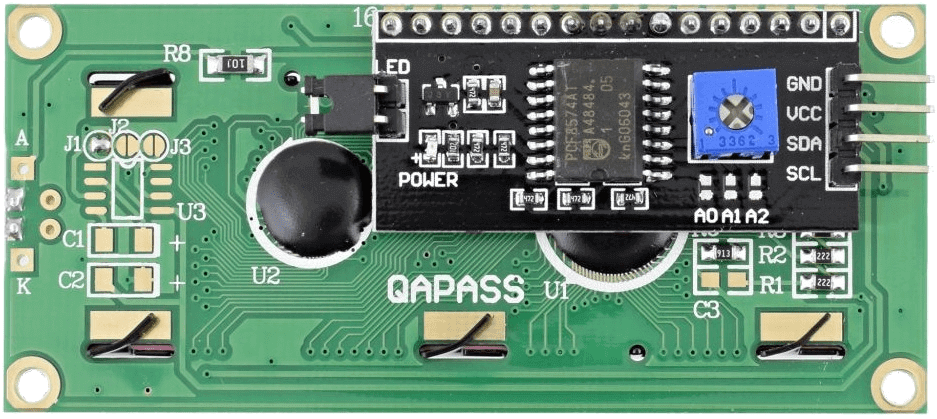
\includegraphics[width=0.9\linewidth]{images/krb/zadni-cast-lcd-displeje-s-expanderem-pcf8574.png}
  \caption{Zadní část displeje s I$^2$C expandérem PCF8574.}
  \label{fig:zadni-cast-lcd-displeje-s-expanderem-pcf857}
\end{subfigure}
\caption[LCD displej pro zobrazování teplot ze zásobníku otopné vody.]{LCD displej pro zobrazování teplot ze zásobníku otopné vody \cite{lcd-displej}.}
\label{fig:lcd-displej}
\end{figure}

\subsubsection{Realizovaná DPS signalizace u krbů}
Výše popsané části jsou realizované na DPS (obrázek \ref{fig:dps-led-ochrany-u-krbu-spodek}, \ref{fig:dps-led-ochrany-u-krbu-vrsek}, \ref{fig:dps-led-ochrany-u-krbu-kabely}). Deska byla vlastnoručně navržena, vyrobena a osazena. Je aplikován ochranný lak. Celkové schéma zapojení je v příloze \ref{app:schemata-ostatni}.

\begin{figure}[H]
    \centering
    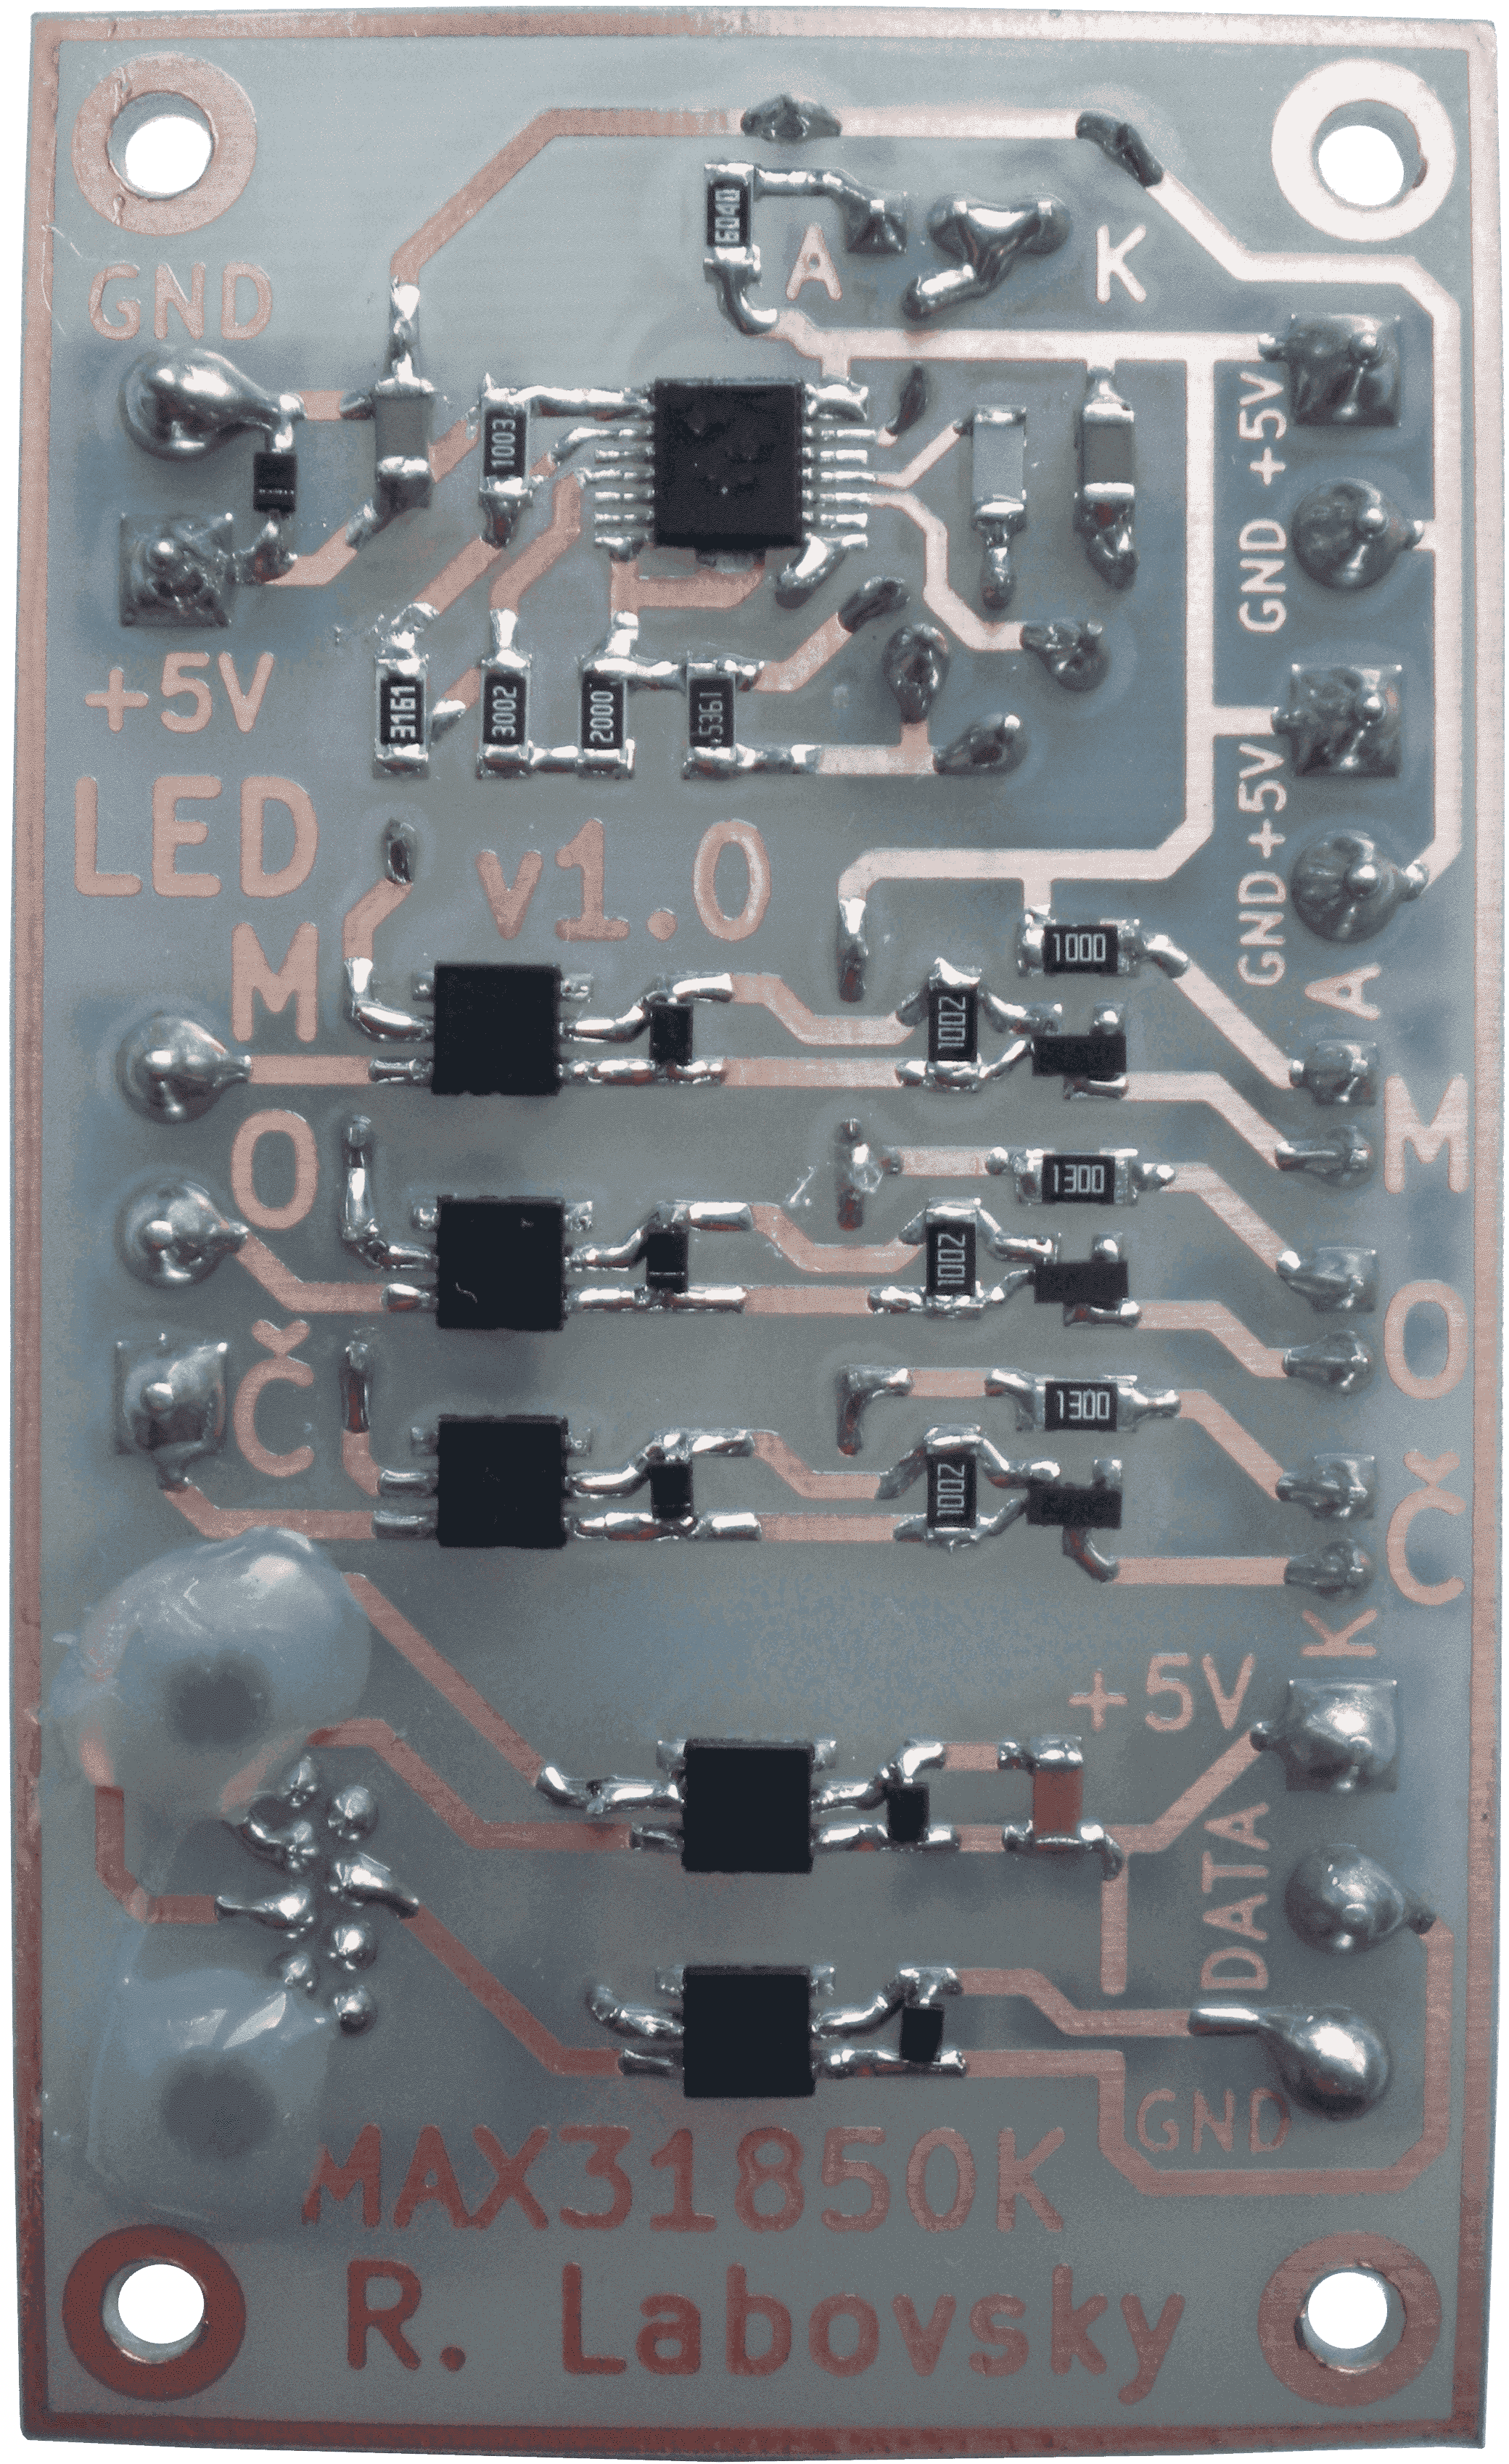
\includegraphics[width=\textwidth]{images/krb/dps-led-ochrany-u-krbu-spodek.png}
    \caption{Spodní část DPS pro signalizaci u krbu.}
    \label{fig:dps-led-ochrany-u-krbu-spodek}
\end{figure}

\begin{figure}[H]
    \centering
    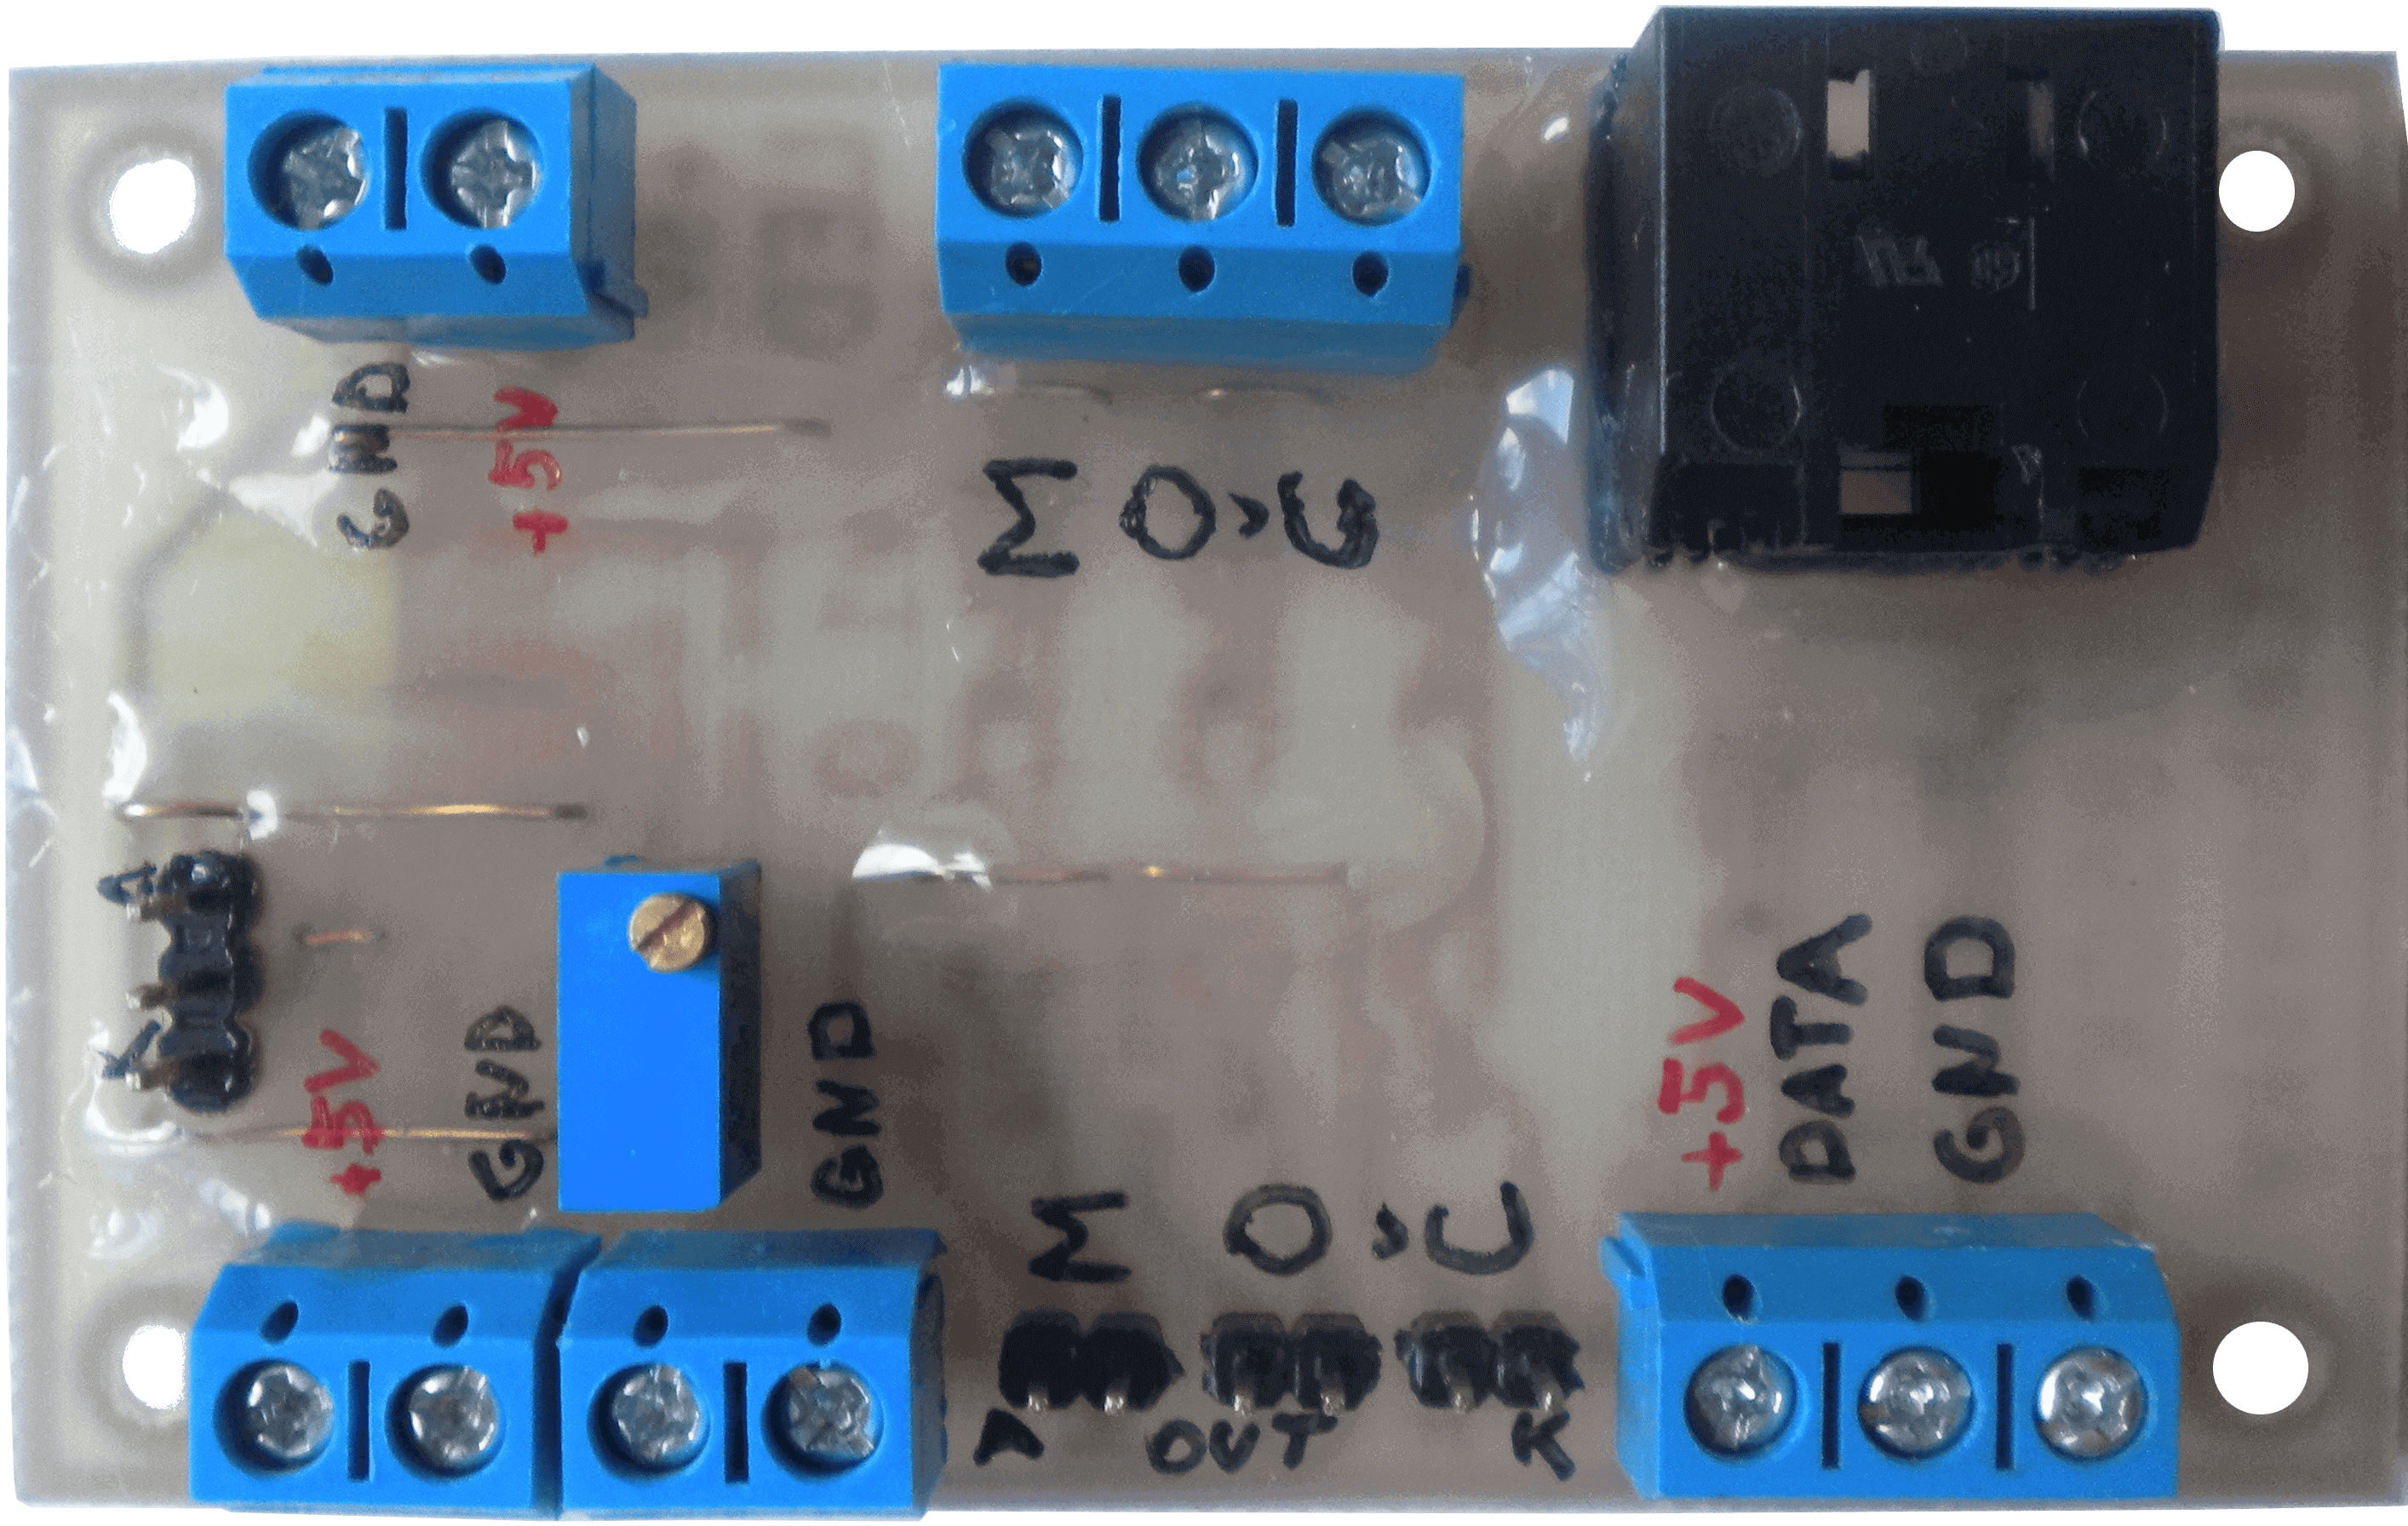
\includegraphics[width=\textwidth]{images/krb/dps-led-ochrany-u-krbu-vrsek.png}
    \caption{Horní část DPS pro signalizaci u krbu.}
    \label{fig:dps-led-ochrany-u-krbu-vrsek}
\end{figure}

\begin{figure}[H]
    \centering
    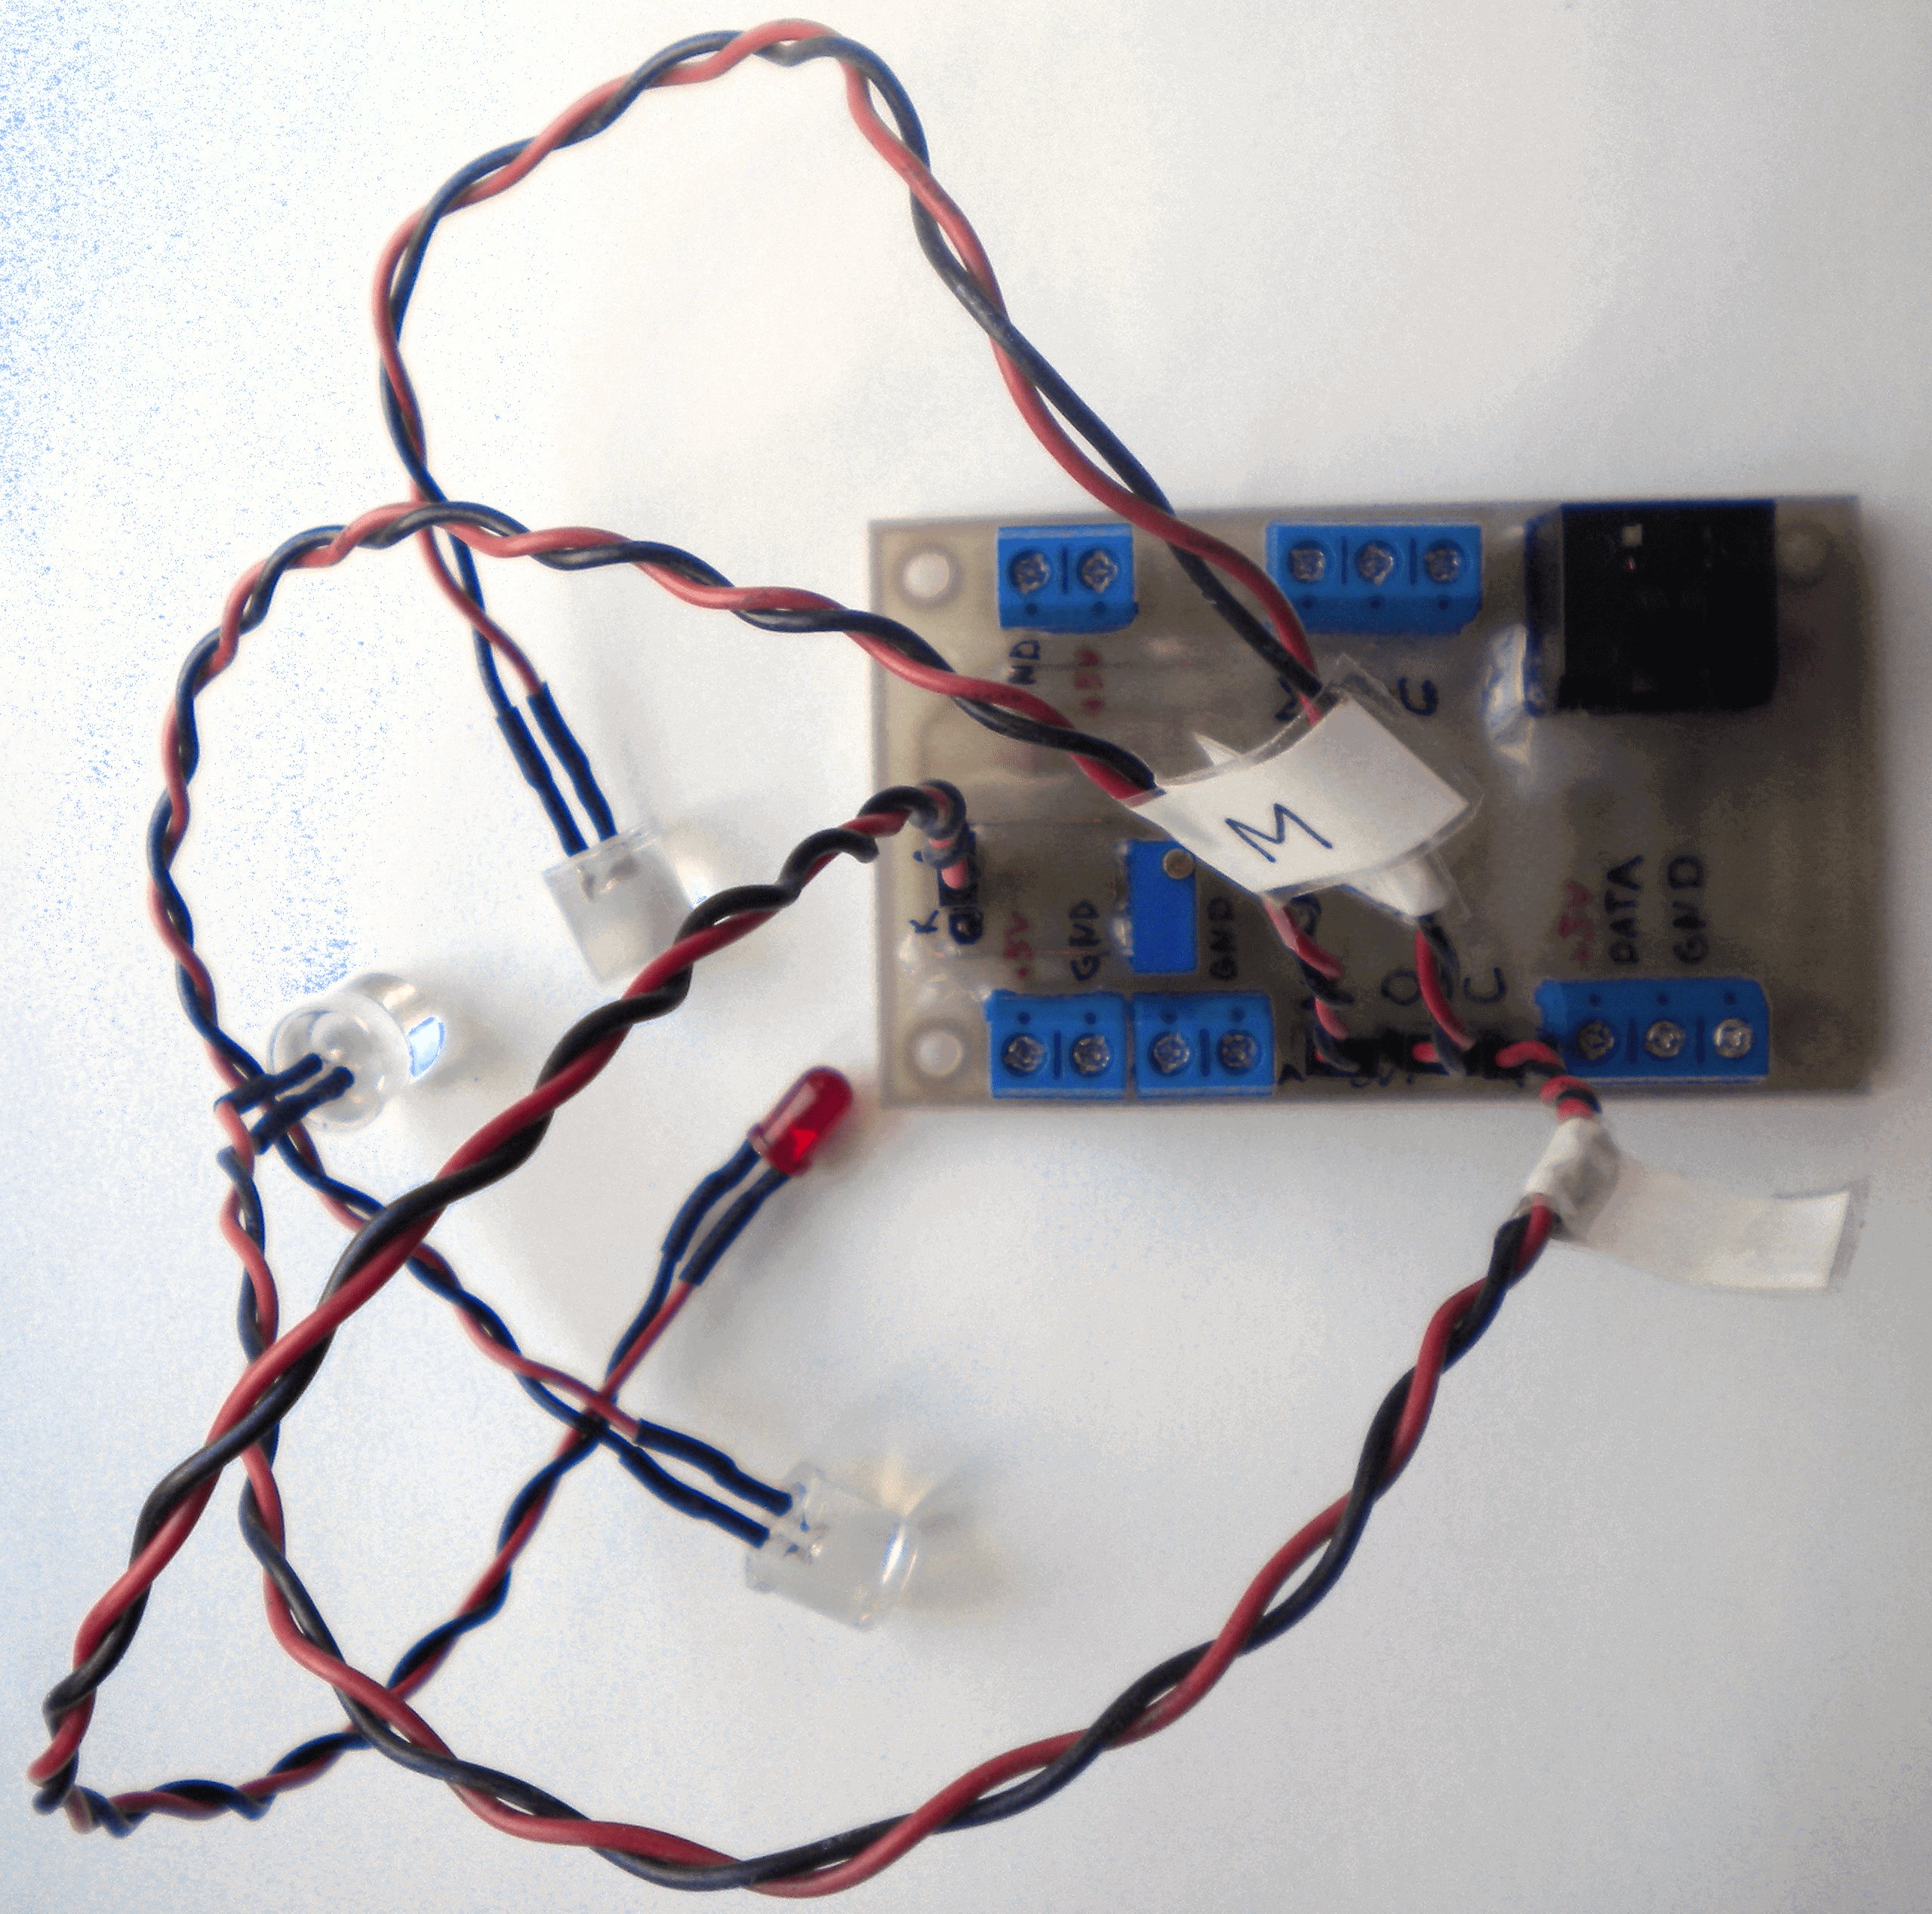
\includegraphics[width=0.95\textwidth]{images/krb/dps-led-ochrany-u-krbu-kabely.png}
    \caption{DPS včetně signalizačních LED.}
    \label{fig:dps-led-ochrany-u-krbu-kabely}
\end{figure}

\subsubsection{Instalační krabice}
Všechna elektronika je umístěna do ochranné instalační krabice (obrázek \ref{fig:instalacni-krabice-vnitrek-krb}). Do krabice vstupují dva vodiče pro napětí 5 V a zem, tři kabely pro ovládání signalizačních LED, UTP kabel se sběrnicí 1-Wire pro teplotní senzor (termočlánek) a I$^2$C sběrnicí. Na obrázku \ref{fig:zadni-cast-krytu-vika-instalacni-krabice-krb} je zobrazena zadní část víka instalační krabice s uchycením signalizačních LED a LCD displeje. Na obrázku \ref{fig:predni-cast-krytu-vika-instalacni-krabice-krb} je přední část víka instalační krabice. Takto zkompletovaná instalační krabice je umístěna u krbu ve sklepě, v přízemí a v patře.

\begin{figure}[H]
    \centering
    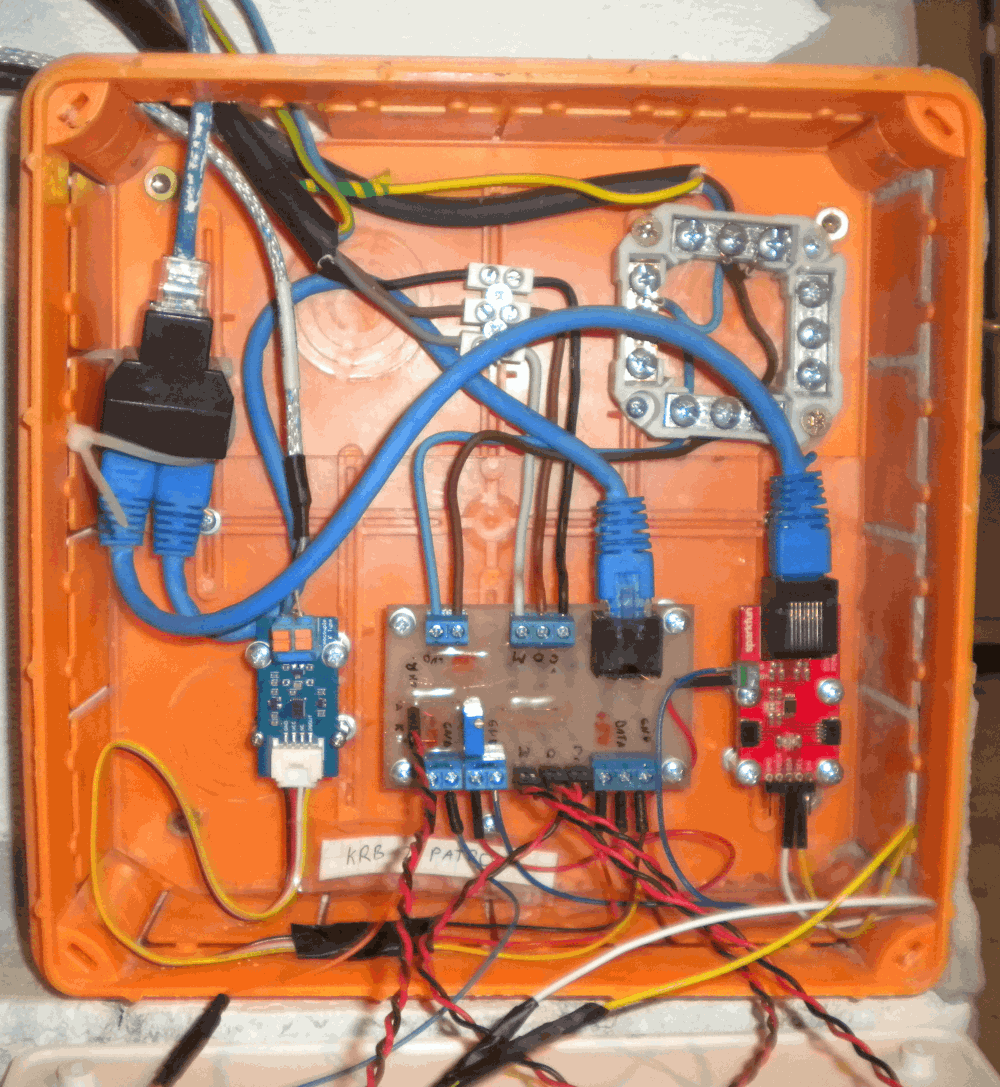
\includegraphics[width=0.6\textwidth]{images/krb/instalacni-krabice-vnitrek-krb.png}
    \caption{Instalační krabice s jednotlivými moduly.}
    \label{fig:instalacni-krabice-vnitrek-krb}
\end{figure}

\begin{figure}[H]
    \centering
    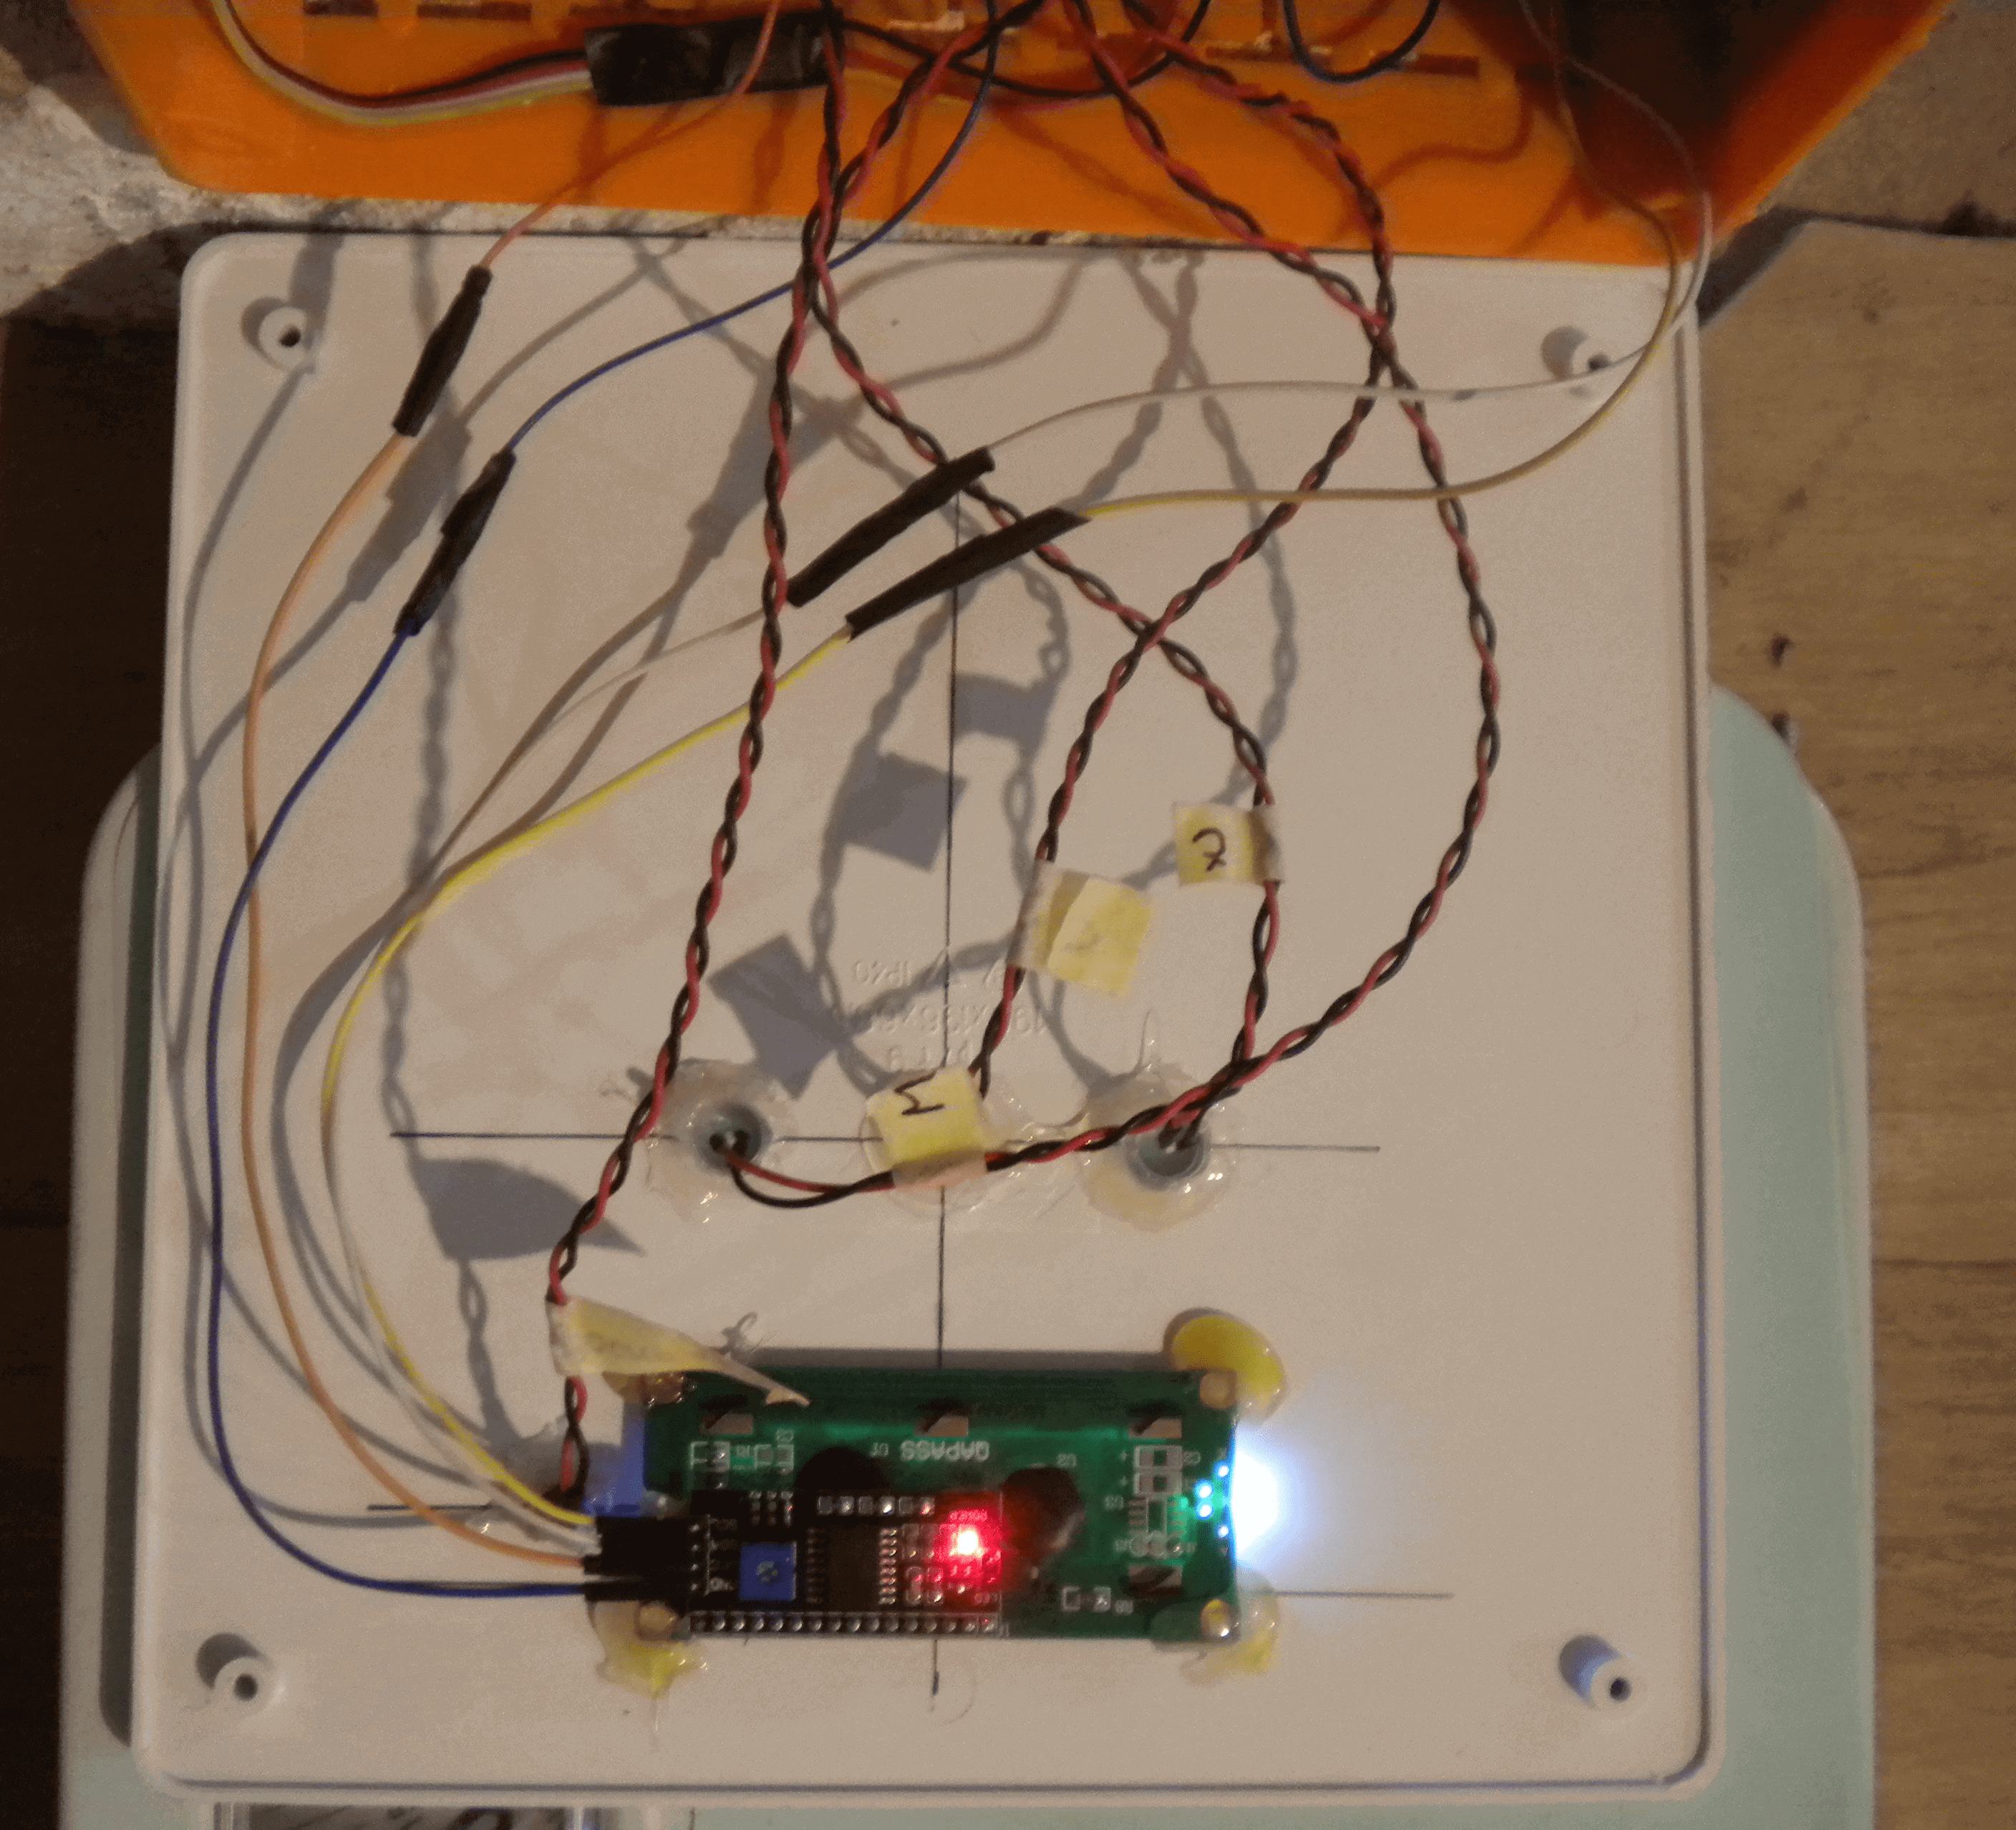
\includegraphics[width=0.6\textwidth]{images/krb/zadni-cast-krytu-vika-instalacni-krabice-krb.png}
    \caption{Zadní část instalační krabice.}
    \label{fig:zadni-cast-krytu-vika-instalacni-krabice-krb}
\end{figure}

\begin{figure}[H]
    \centering
    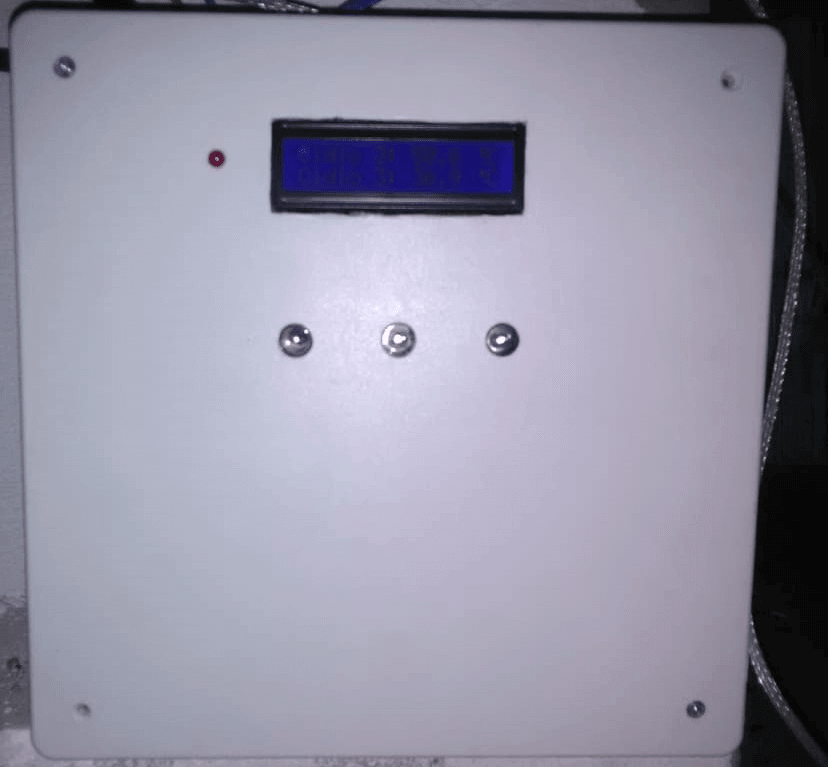
\includegraphics[width=0.6\textwidth]{images/krb/predni-cast-krytu-vika-instalacni-krabice-krb.png}
    \caption[Víko instalační krabice.]{Víko instalační krabice. Osazený LCD displej, signalizačních LED (zleva modrá, oranžová a červená) a LED pro aktivování elektronické pojistky (červená LED vlevo od displeje).}
    \label{fig:predni-cast-krytu-vika-instalacni-krabice-krb}
\end{figure}


\section{Realizace 1-Wire sběrnice u zásobníku otopné vody}
Na obrázku \ref{fig:dps-1-wire-sbernice-u-zasobniku-otopne-vody} je realizovaná DPS pro teplotní senzory u zásobníku otopné vody. Deska byla vlastnoručně navržena, vyrobena a osazena. Je aplikován ochranný lak. Princip zapojení včetně ochrana na napájecí i datové části je popsán v~části \ref{sec:dps-se-vstupy-vystupy-pro-raspberry-pi} (datová část 1-Wire sběrnice). Na obrázku \ref{fig:instalacni-krabice-cidla-u-zasobniku-otopne-vody} je vidět horní část DPS vložená do instalační krabice. Celkově je zde k dispozici 6~pozic pro upevnění přes svorkovnice teplotní senzory. V současnosti jsou zde napojeny 3 teplotní senzory (pro snímání teplot z horní, střední a spodní části zásobníku otopné vody). Na obrázku \ref{fig:ds18b20-ochrana} je teplotní senzor DS18B20 v~pouzdře TO-92 připevněn na UTP kabel a zataven plastovou hmotou na níž je následně nanesena smršťovací ochranná bužírka. Na obrázku \ref{fig:zasobnik-otopné-vody} jsou vyznačená místa s umístěním teplotních senzorů. Celkové schéma zapojení je v příloze \ref{app:schemata-ostatni}.

\begin{figure}[H]
    \centering
    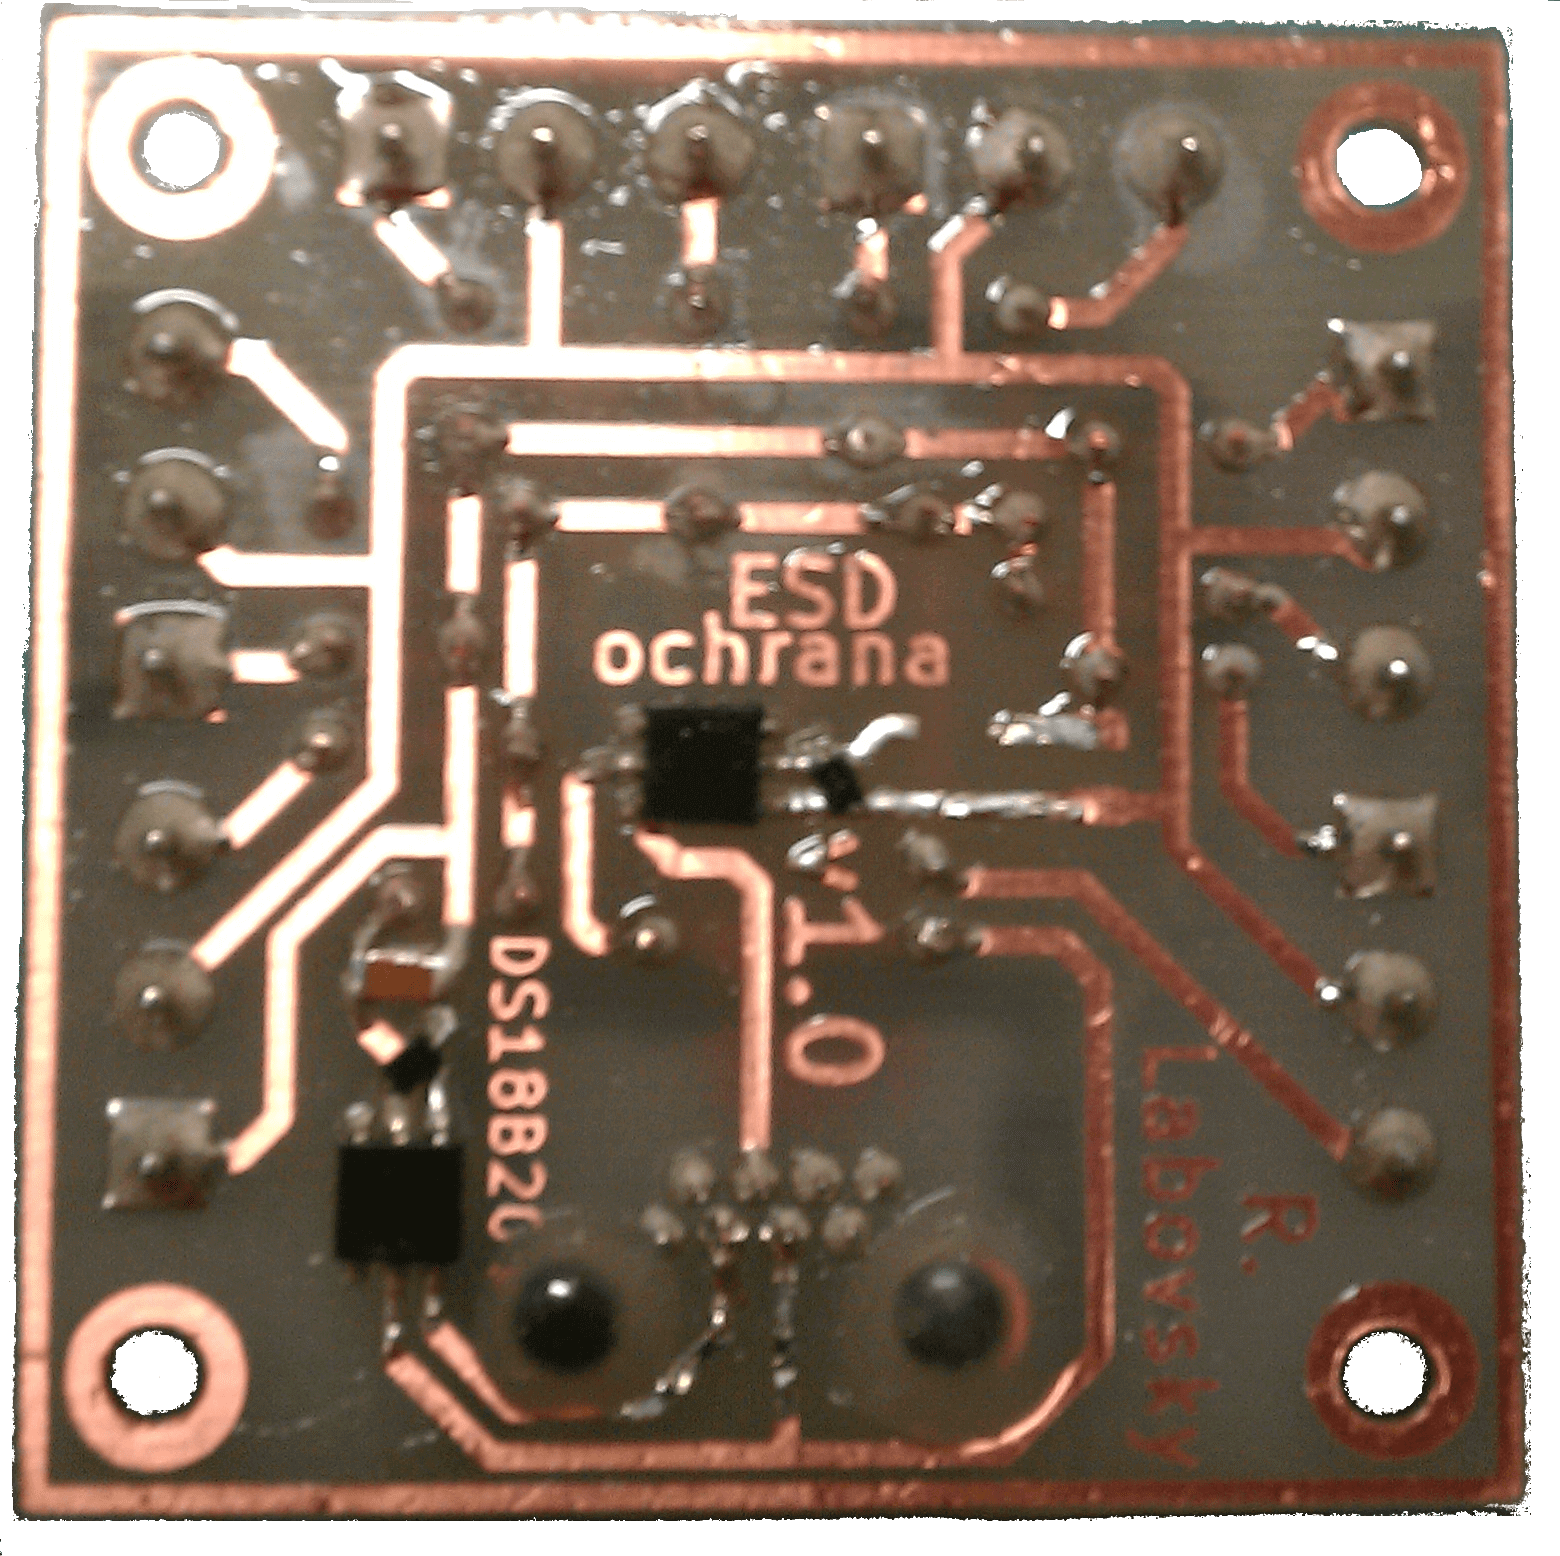
\includegraphics[width=0.6\textwidth]{images/zasobnik-otopne-vody/dps-1-wire-sbernice-u-zasobniku-otopne-vody.png}
    \caption{Realizovaná DPS pro teplotní senzory 1-Wire sběrnice u zásobníku otopné vody.}
    \label{fig:dps-1-wire-sbernice-u-zasobniku-otopne-vody}
\end{figure}

\begin{figure}[H]
    \centering
    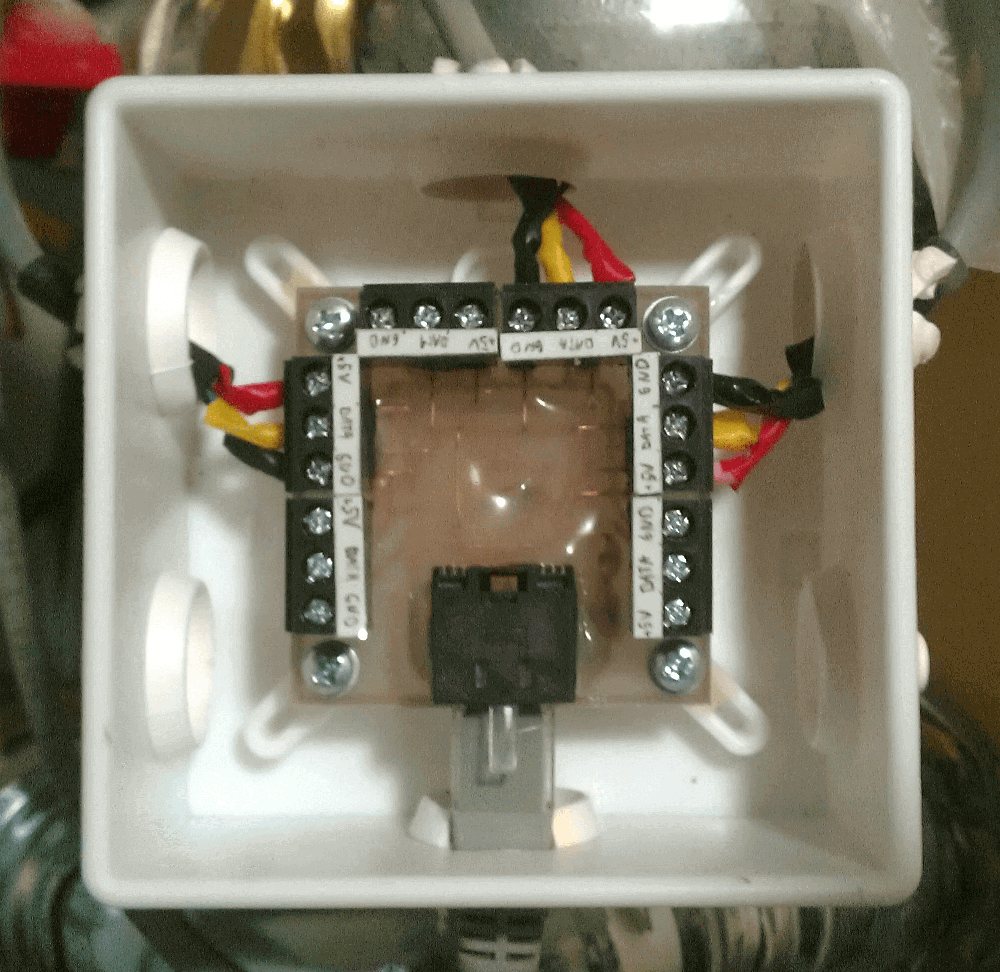
\includegraphics[width=0.6\textwidth]{images/zasobnik-otopne-vody/instalacni-krabice-cidla-u-zasobniku-otopne-vody.png}
    \caption{Horní část DPS umístěná do instalační krabice.}
    \label{fig:instalacni-krabice-cidla-u-zasobniku-otopne-vody}
\end{figure}

\begin{figure}[H]
    \centering
    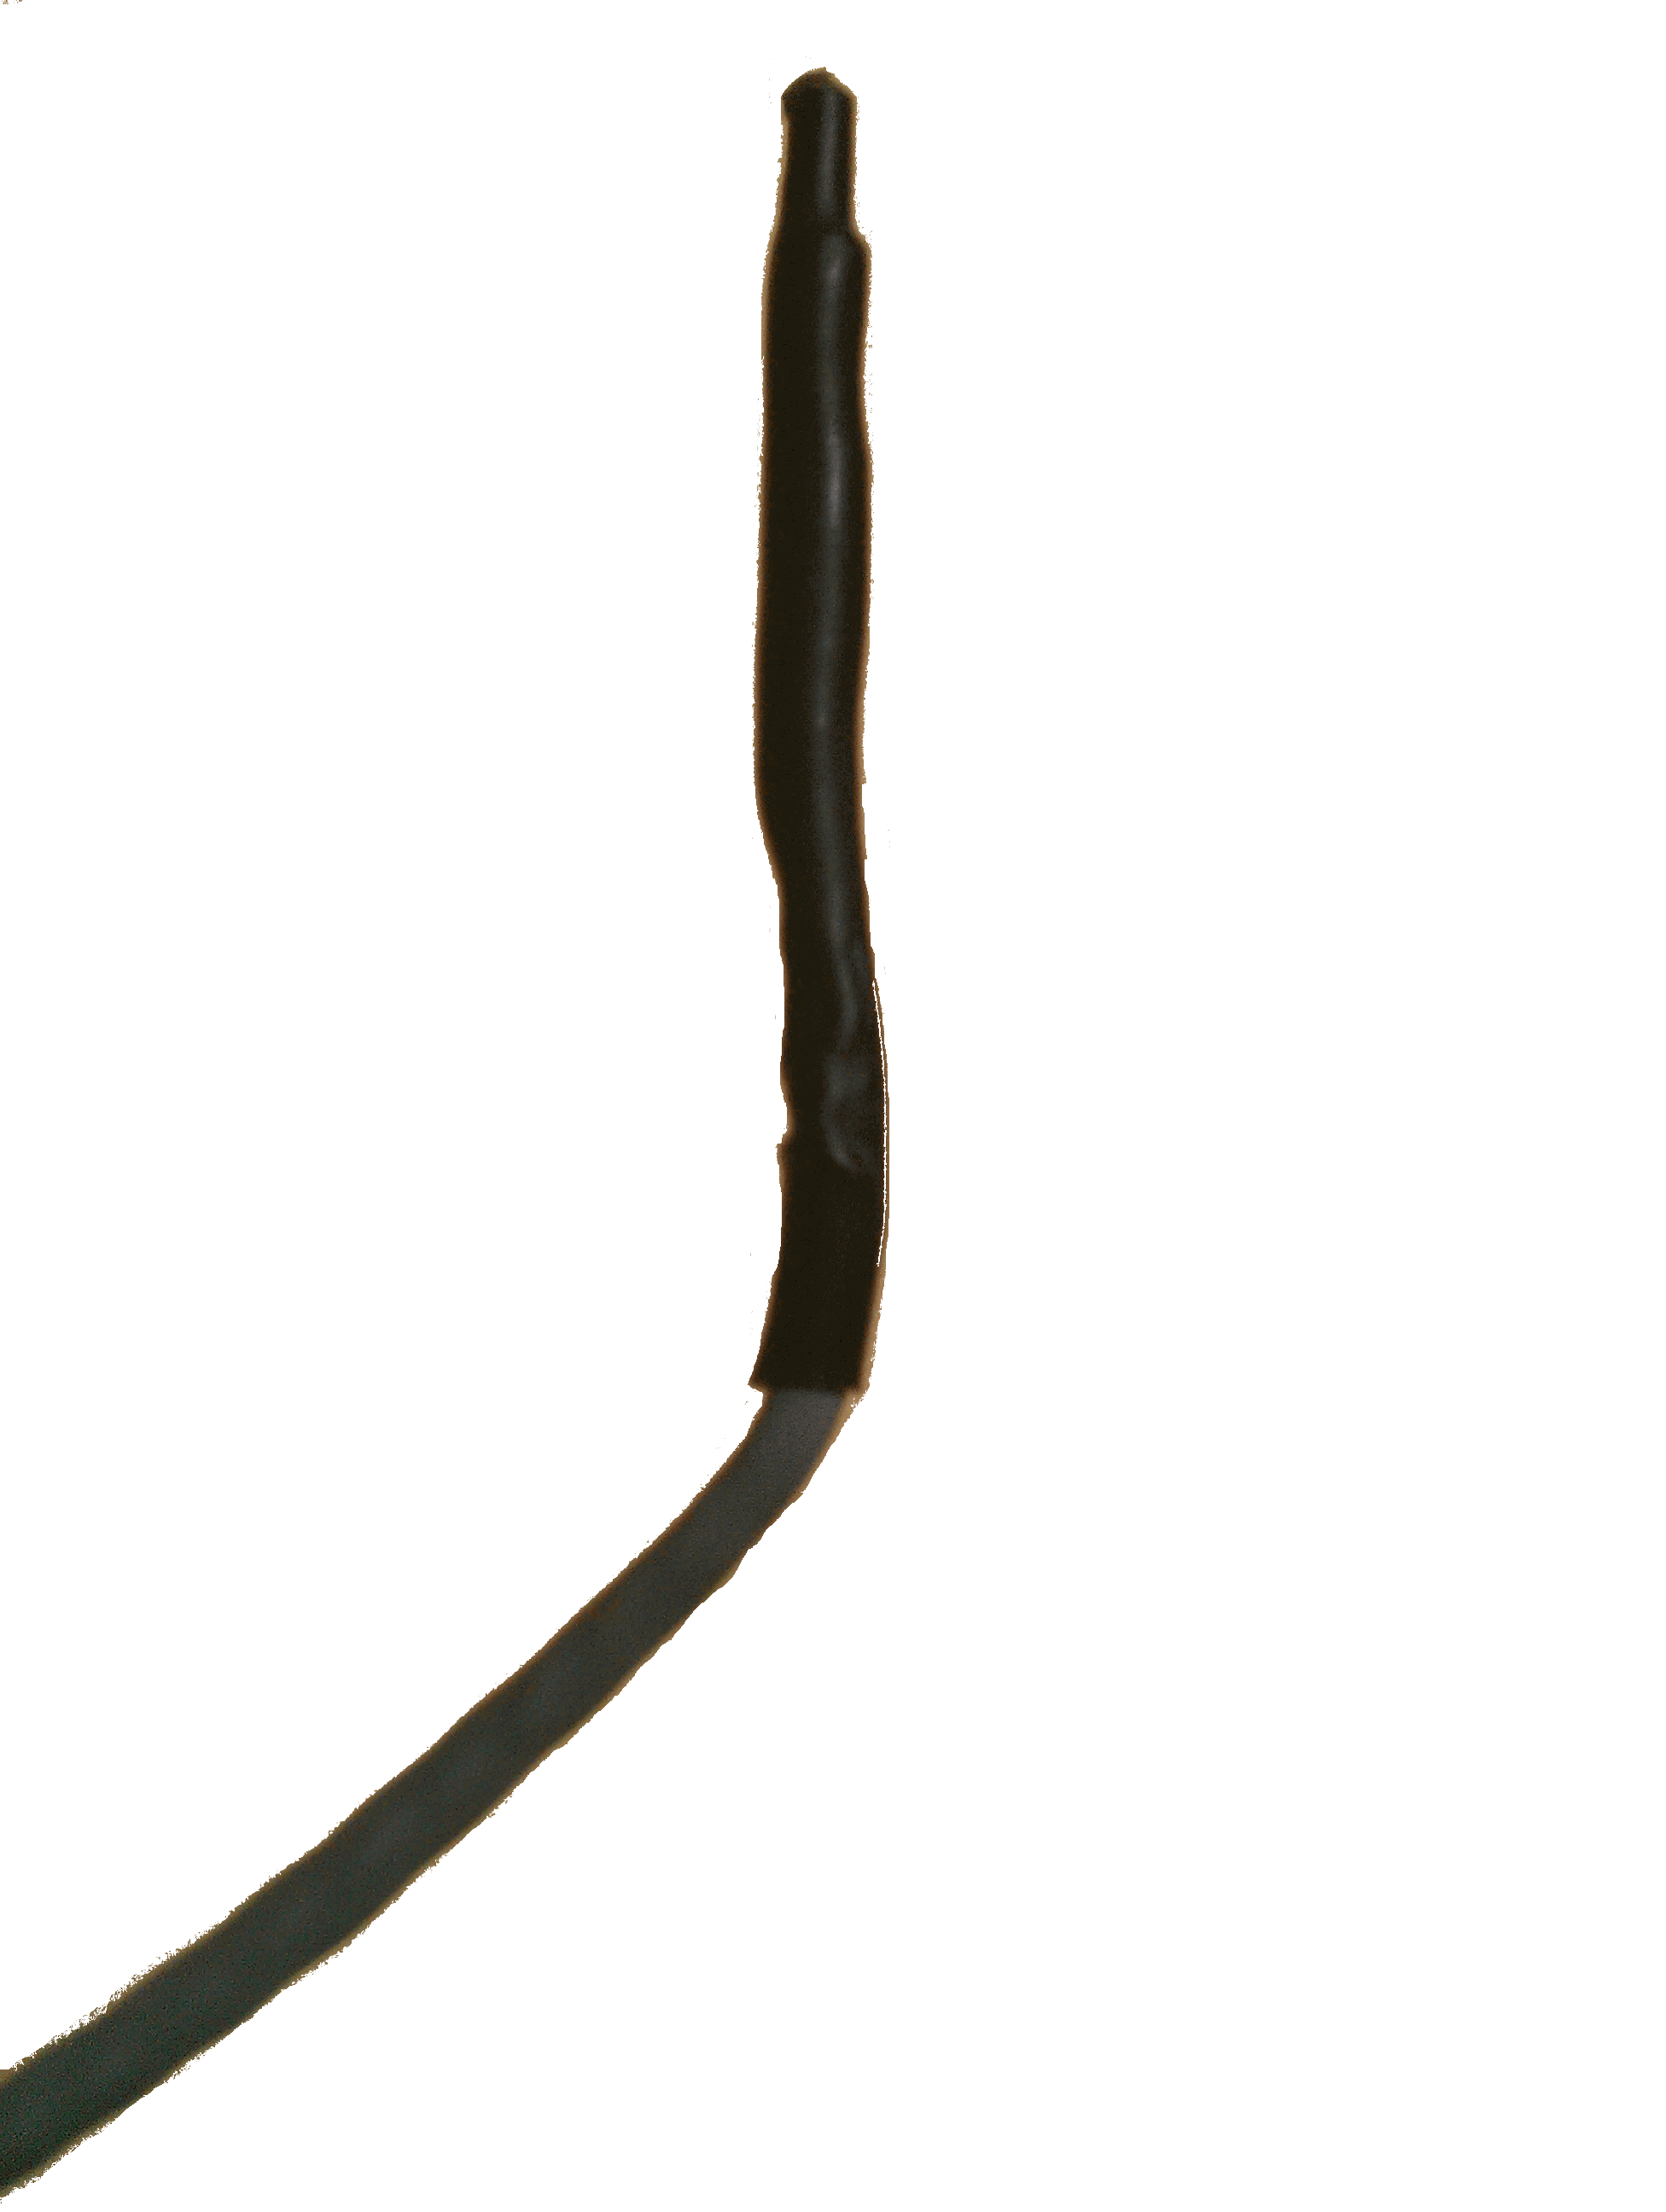
\includegraphics[width=0.6\textwidth]{images/zasobnik-otopne-vody/ds18b20-ochrana.png}
    \caption{Teplotní senzor DS18B20 v~ochranném pouzdře.}
    \label{fig:ds18b20-ochrana}
\end{figure}

\begin{figure}[H]
    \centering
    \includegraphics[width=\textwidth]{images/zasobnik-otopne-vody/zasobnik-otopné-vody.png}
    \caption[Zásobník otopné vody.]{Zásobník otopné vody. Červené kroužky označují místa teplotních senzorů.}
    \label{fig:zasobnik-otopné-vody}
\end{figure}